\documentclass[conference,a4paper,twoside]{IEEEtran}
\usepackage[utf8]{inputenc}
\usepackage{amsmath}
\usepackage{amsfonts}
\usepackage{amssymb}
\usepackage{graphicx}
\usepackage{url}
\usepackage{hyperref}
\usepackage{subcaption}
\RequirePackage[date=terse,isbn=true,doi=true,url=false,urldate=iso8601,maxbibnames=9,backref=false,backend=bibtex]{biblatex}
\addbibresource{securityupdates.bib}
\renewcommand{\bibfont}{\small}

\AtEveryBibitem{% Clean up the bibtex rather than editing it
 \clearname{editor} % remove editors
}

\author{Daniel R.\ Thomas, Daniel T.\ Wagner, Alastair R.\ Beresford and Andrew Rice}

\newcommand{\daNumDataPoints}{153 Billion}
\newcommand{\daNumStartedApps}{122\,000}
\newcommand{\daNumInstalledApps}{175\,000}
\newcommand{\daNumVulnsUsed}{11}
\newcommand{\daSigNumDevices}{100}
\newcommand{\daSigNumDays}{100}
\newcommand{\daNumManufacturers}{261}
\newcommand{\daNumSigManufacturers}{9}
\newcommand{\daNumModels}{2\,380}
\newcommand{\daNumSigModels}{15}
\newcommand{\daOSVersionPercValidLines}{99.5\%}
\newcommand{\daOSTotalDaysData}{1\,140\,000}
\newcommand{\daMeanInsecurityPerc}{$87.3 \pm 0.0\%$}
\newcommand{\daMeanOutstandingVulnerabilities}{0.637}
\newcommand{\daUpdatedness}{$0.0558 \pm 0.0002$}
\newcommand{\daSecurityScore}{$2.75 \pm 0.00$}
\newcommand{\daNumFullVersions}{1\,140}
\newcommand{\daNumOSVersions}{45}
\newcommand{\daNumSigOSVersions}{23}
\newcommand{\daNumAPIVersions}{15}
\newcommand{\daNumFullVersionUpdates}{4\,220}
\newcommand{\daNumOSVersionUpdates}{3\,560}
\newcommand{\daNumFullOnlyVersionUpdates}{640}
\newcommand{\daNumSecurityUpdates}{1\,110}
\newcommand{\daNumPossibleSecurityUpdates}{2\,140}
\newcommand{\daTabSecScoresmanufacturer}{\begin{table} \centering \begin{tabular}{l|c|c|c|c} Name & $f$ & $u$ & $m$ & \textbf{Security score} \\ &&&& (out of 10) \\ \hline LG & $0.12 \pm 0.00$ & $0.32 \pm 0.00$ & 0.74 & $3.38 \pm 0.01$ \\  Motorola & $0.16 \pm 0.00$ & $0.13 \pm 0.00$ & 0.77 & $2.93 \pm 0.01$ \\  other & $0.13 \pm 0.00$ & $0.06 \pm 0.00$ & 0.64 & $2.75 \pm 0.00$ \\  Samsung & $0.14 \pm 0.00$ & $0.05 \pm 0.00$ & 0.71 & $2.67 \pm 0.00$ \\  Sony & $0.13 \pm 0.00$ & $0.18 \pm 0.00$ & 1.02 & $2.64 \pm 0.01$ \\  HTC & $0.14 \pm 0.00$ & $0.09 \pm 0.00$ & 0.89 & $2.55 \pm 0.00$ \\  asus & $0.15 \pm 0.00$ & $0.56 \pm 0.01$ & 6.06 & $2.30 \pm 0.02$ \\  Symphony & $0.00 \pm 0.00$ & $0.04 \pm 0.00$ & 4.79 & $0.19 \pm 0.00$ \\  walton & $0.00 \pm 0.00$ & $0.04 \pm 0.00$ & 5.79 & $0.14 \pm 0.01$ \\ \end{tabular} \caption{Security scores for manufacturers} \label{tab:sec_manufacturer} \end{table}}
\newcommand{\daTabSecScoresmodel}{\begin{table} \centering \begin{tabular}{l|c|c|c|c} Name & $f$ & $u$ & $m$ & \textbf{Security score} \\ &&&& (out of 10) \\ \hline Galaxy Nexus & $0.53 \pm 0.00$ & $0.53 \pm 0.01$ & 1.53 & $4.80 \pm 0.03$ \\  Nexus 4 & $0.23 \pm 0.00$ & $0.82 \pm 0.01$ & 6.06 & $3.39 \pm 0.04$ \\  Nexus 7 & $0.19 \pm 0.00$ & $0.74 \pm 0.01$ & 5.92 & $3.02 \pm 0.04$ \\  other & $0.13 \pm 0.00$ & $0.12 \pm 0.00$ & 0.64 & $2.94 \pm 0.00$ \\  Desire HD & $0.08 \pm 0.00$ & $0.05 \pm 0.00$ & 0.39 & $2.91 \pm 0.02$ \\  HTC Sensation & $0.36 \pm 0.00$ & $0.01 \pm 0.01$ & 1.59 & $2.47 \pm 0.02$ \\  GT-I9100 & $0.22 \pm 0.00$ & $0.02 \pm 0.00$ & 1.20 & $2.33 \pm 0.01$ \\  HTC Desire S & $0.02 \pm 0.00$ & $0.02 \pm 0.00$ & 1.00 & $1.75 \pm 0.01$ \\  GT-N7000 & $0.25 \pm 0.00$ & $0.00 \pm 0.00$ & 2.52 & $1.43 \pm 0.02$ \\  GT-P1000 & $0.01 \pm 0.00$ & $0.00 \pm 0.01$ & 1.73 & $0.94 \pm 0.02$ \\  GT-I9300 & $0.15 \pm 0.00$ & $0.01 \pm 0.00$ & 6.15 & $0.64 \pm 0.01$ \\  GT-I9505 & $0.00 \pm 0.00$ & $0.18 \pm 0.00$ & 6.77 & $0.55 \pm 0.01$ \\  GT-N7100 & $0.07 \pm 0.00$ & $0.00 \pm 0.01$ & 6.91 & $0.28 \pm 0.02$ \\  HTC Desire HD & $0.00 \pm 0.00$ & $0.00 \pm 0.01$ & 3.05 & $0.27 \pm 0.02$ \\ \end{tabular} \caption{Security scores for models} \label{tab:sec_model} \end{table}}
\newcommand{\daTabSecScoressummary}{\begin{table} \centering \begin{tabular}{l|c|c|c|c} Name & $f$ & $u$ & $m$ & \textbf{Security score} \\ &&&& (out of 10) \\ \hline nexus & $0.36 \pm 0.00$ & $0.51 \pm 0.00$ & 0.68 & $5.01 \pm 0.01$ \\  notnexus & $0.12 \pm 0.00$ & $0.04 \pm 0.00$ & 0.64 & $2.67 \pm 0.00$ \\ \end{tabular} \caption{Security scores for nexus} \label{tab:sec_summary} \end{table}}
\newcommand{\daUpdatednessPerc}{$5.58 \pm 0.02\%$}
\newcommand{\daNumOSDevices}{19\,000}
\newcommand{\daSigNumDevicesDay}{20}
\newcommand{\daSigNumDeviceDays}{10\,000}
\newcommand{\daTabAndVulns}{\begin{table} \centering \begin{tabular}{l|c|l} Vulnerability & Date known & How known \\ \hline KillingInTheNameOf psneuter ashmem & 2010-07-13 & Fixed on \\ exploid udev & 2010-07-15 & Discovered on \\ RageAgainstTheCage adb & 2010-08-21 & Discovered on \\ levitator & 2011-03-10 & Discovered on \\ Gingerbreak & 2011-04-18 & Fixed on \\ zergRush & 2011-10-06 & Discovered on \\ APK duplicate file & 2013-02-18 & Discovered on \\ APK unchecked name & 2013-06-30 & Discovered on \\ APK unsigned shorts & 2013-07-03 & Fixed on \\ keystore buffer & 2013-09-09 & Discovered on \\ TwerkMyMoto & 2013-11-24 & Discovered on \\ vold asec & 2014-01-27 & Fixed on \\\end{tabular} \caption{Root equivalent vulnerabilities in Android} \label{tab:andvulns} \end{table}}
\newcommand{\daOSYearsOfData}{3}
\newcommand{\daSecScoreBestmanufacturer}{LG}
\newcommand{\daSecScoreWorstmanufacturer}{walton}
\newcommand{\daSecScoreBestmodel}{Galaxy Nexus}
\newcommand{\daSecScoreWorstmodel}{HTC Desire HD A9191}
\newcommand{\daSecScoreBestsummary}{nexus}
\newcommand{\daSecScoreWorstsummary}{notnexus}
\newcommand{\daSecScoreBestmanufacturerScore}{$3.38 \pm 0.01$}
\newcommand{\daSecScoreWorstmanufacturerScore}{$0.139 \pm 0.006$}
\newcommand{\daSecScoreBestmodelScore}{$4.8 \pm 0.0$}
\newcommand{\daSecScoreWorstmodelScore}{$0.274 \pm 0.020$}
\newcommand{\daSecScoreBestsummaryScore}{$4.1 \pm 0.0$}
\newcommand{\daSecScoreWorstsummaryScore}{$2.9 \pm 0.0$}
\newcommand{\daVulnFree}{$0.127 \pm 0.000$}
\newcommand{\daAdbEnabledPerc}{$19.5 \pm 0.0\%$}
\newcommand{\daNumUpdatesUpgrades}{3\,330}
\newcommand{\daNumUpdatesDowngrades}{147}
\newcommand{\daPercUpdatesDowngrades}{$3.58 \pm 0.3\%$}
\newcommand{\daStartDate}{2011-07-01}
\newcommand{\daEndDate}{2014-11-07}
\newcommand{\daNumOperators}{1\,390}
\newcommand{\daTabSecScoresoperator}{\begin{table} \centering \begin{tabular}{l|c|c|c|c} Name & $f$ & $u$ & $m$ & \textbf{Security score} \\ &&&& (out of 10) \\ \hline O2 uk & $0.25 \pm 0.00$ & $0.12 \pm 0.00$ & 0.37 & $3.79 \pm 0.01$ \\  T-Mobile & $0.19 \pm 0.00$ & $0.18 \pm 0.00$ & 0.48 & $3.57 \pm 0.01$ \\  Orange & $0.21 \pm 0.00$ & $0.09 \pm 0.00$ & 0.39 & $3.52 \pm 0.02$ \\  Sprint & $0.18 \pm 0.00$ & $0.11 \pm 0.00$ & 0.44 & $3.41 \pm 0.01$ \\  3 & $0.15 \pm 0.00$ & $0.09 \pm 0.00$ & 0.49 & $3.15 \pm 0.01$ \\  AT\&T & $0.12 \pm 0.00$ & $0.08 \pm 0.00$ & 0.43 & $3.08 \pm 0.01$ \\  Vodafone uk & $0.13 \pm 0.00$ & $0.10 \pm 0.00$ & 0.52 & $3.07 \pm 0.01$ \\  Verizon & $0.18 \pm 0.00$ & $0.09 \pm 0.00$ & 0.81 & $2.82 \pm 0.01$ \\  unknown & $0.10 \pm 0.00$ & $0.22 \pm 0.00$ & 1.08 & $2.57 \pm 0.01$ \\  n Telenor & $0.03 \pm 0.00$ & $0.10 \pm 0.00$ & 1.42 & $1.59 \pm 0.01$ \\  Airtel & $0.06 \pm 0.00$ & $0.03 \pm 0.00$ & 1.93 & $1.10 \pm 0.01$ \\  Grameenphone & $0.01 \pm 0.00$ & $0.02 \pm 0.00$ & 1.99 & $0.80 \pm 0.00$ \\  Robi & $0.00 \pm 0.00$ & $0.04 \pm 0.00$ & 2.19 & $0.73 \pm 0.01$ \\  banglalink & $0.00 \pm 0.00$ & $0.03 \pm 0.00$ & 2.90 & $0.40 \pm 0.00$ \\ \end{tabular} \caption{Security scores for operators} \label{tab:sec_operator} \end{table}}
\newcommand{\daSecScoreBestoperator}{O2 uk}
\newcommand{\daSecScoreBestoperatorScore}{$3.79 \pm 0.01$}
\newcommand{\daSecScoreWorstoperator}{banglalink}
\newcommand{\daSecScoreWorstoperatorScore}{$0.4 \pm 0.0$}
\newcommand{\daNumSigOperators}{14}
\newcommand{\daMonthsDevices}{1\,600}
\newcommand{\daMonths}{6}
\newcommand{\daSigVersionPerc}{1\%}
\newcommand{\daSigVersionDays}{10}
\newcommand{\daNumDeviceDataDevices}{50}
\newcommand{\daNumSigFullVersions}{83}
\newcommand{\daSecScoreBestmanufacturerNumFullVersions}{104}
\newcommand{\daSecScoreworstmanufacturerNumFullVersions}{239}
\newcommand{\daSecScoreBestmodelNumFullVersions}{49}
\newcommand{\daSecScoreworstmodelNumFullVersions}{2}
\newcommand{\daSecScoreBestsummaryNumFullVersions}{73}
\newcommand{\daSecScoreworstsummaryNumFullVersions}{1057}
\newcommand{\daSecScoreBestoperatorNumFullVersions}{88}
\newcommand{\daSecScoreworstoperatorNumFullVersions}{89}
\newcommand{\daSecScoreWorstmanufacturerNumFullVersions}{20}
\newcommand{\daSecScoreWorstmodelNumFullVersions}{2}
\newcommand{\daSecScoreWorstsummaryNumFullVersions}{1103}
\newcommand{\daSecScoreWorstoperatorNumFullVersions}{59}
\newcommand{\daFullDeployedAt}{95\%}
\newcommand{\daOSCurveFitParamFirst}{87.5}
\newcommand{\daOSCurveFitParamSecond}{\num{0.00315}}
\newcommand{\daOSCurveFitRMSE}{0.114}
\newcommand{\daAPICurveFitParamFirst}{110}
\newcommand{\daAPICurveFitParamSecond}{\num{0.00315}}
\newcommand{\daAPICurveFitRMSE}{0.116}
\newcommand{\daOSCurvePolyRMSE}{0.115}
\newcommand{\daOSCurveSplineRMSE}{0.115}
\newcommand{\daOSCurveHalfDeployed}{$308 \pm 81$}
\newcommand{\daOSCurveFullDeployed}{$1\,040 \pm 236\,000$}
\newcommand{\daAPICurvePolyRMSE}{0.117}
\newcommand{\daAPICurveSplineRMSE}{0.117}
\newcommand{\daAPICurveHalfDeployed}{$330 \pm 84$}
\newcommand{\daAPICurveFullDeployed}{$1\,060 \pm 236\,000$}
\newcommand{\daVulnAPKDuplicateFileOctoberPerc}{91.5\%}
\newcommand{\daNumUpdatesBigUpgrades}{778}
\newcommand{\daNumUpdatesSkippedBig}{3}
\newcommand{\daPercBigUpgrades}{$18.9 \pm 0.7\%$}
\newcommand{\daUpdatesPerYear}{$1.35 \pm 0.02$}
\newcommand{\daOSMonthsOfData}{40}
\newcommand{\daMeanInsecurityPercNominal}{87.3\%}
\newcommand{\daVulnFreeNominal}{0.127}
\newcommand{\daUpdatednessNominal}{0.0558}
\newcommand{\daUpdatednessPercNominal}{5.58\%}
\newcommand{\daSecurityScoreNominal}{2.75}
\newcommand{\daUpdatesPerYearNominal}{1.35}
\newcommand{\daOSCurveHalfDeployedNominal}{308}
\newcommand{\daOSCurveFullDeployedNominal}{1\,040}
\newcommand{\daAPICurveHalfDeployedNominal}{330}
\newcommand{\daAPICurveFullDeployedNominal}{1\,060}
\newcommand{\daSecScoreBestoperatorScoreNominal}{3.79}
\newcommand{\daSecScoreWorstoperatorScoreNominal}{0.4}
\newcommand{\daSecScoreBestmodelScoreNominal}{4.8}
\newcommand{\daSecScoreWorstmodelScoreNominal}{0.274}
\newcommand{\daAdbEnabledPercNominal}{19.5\%}
\newcommand{\daSecScoreBestmanufacturerScoreNominal}{3.38}
\newcommand{\daSecScoreWorstmanufacturerScoreNominal}{0.139}
\newcommand{\daUpdatesPerMonthPerVersion}{$3.62 \pm 0.06$}
\newcommand{\daNumUpdateFullOnly}{637}
\newcommand{\daVulnZergRushMonthsDefFixDeployed}{27.3}
\newcommand{\daUpdatesPerMonthPerVersionNominal}{3.62}
\newcommand{\daPercBigUpgradesNominal}{18.9\%}
\newcommand{\daPercUpdatesDowngradesNominal}{3.58\%}

\newcommand{\percMarketShare}{XX\%~\cite{TODO}}
\newcommand{\daNumNetworkOperators}{XXX~[\S\ref{sec:results}]}
\newcommand{\daNumDevices}{XXXX}
\newcommand{\daDeviceDays}{XXXXX}
\newcommand{\daMonths}{X}% Number of months for which we have the below number of devices
\newcommand{\daMonthsDevices}{XXX}
\newcommand{\daAdbPerc}{X\%}

\begin{document}
\title{Timeliness of security updates for Android}


% author names and affiliations
% use a multiple column layout for up to three different
% affiliations
\author{
\IEEEauthorblockN{Daniel R. Thomas,
Daniel T. Wagner,
Alastair R. Beresford,
Andrew Rice}
\IEEEauthorblockA{
Computer Laboratory\\
University of Cambridge\\
Cambridge, United Kingdom\\
Firstname.Lastname@cl.cam.ac.uk
}
}


\maketitle

% Hypothesis
% Attempts at fine grained restrictions on running arbitrary code are hampered by updates for security vulnerabilities not reaching users in a timely fashion.

\begin{abstract}
Android is the most popular smartphone platform and seeks to provide better security than popular desktop operating systems through increased compartmentalisation and a permission system for apps.
This security relies on the absence of root privilege exploits which allow apps to bypass protections.
Many such exploits have been found and fixed.
Our hypothesis is that these fixes do not promptly reach the users devices and so much of the time users are running versions of Android known to be vulnerable.
We used Device Analyzer data from over \daOSYearsOfData\ years and \daNumOSDevices\ devices and found that on average over \daMeanInsecurityPerc\ of devices were exposed to known root privilege vulnerabilities and only \daUpdatednessPerc\ of devices run the most recent version of Android.
There was also a period of several months when no devices ran secure versions of Android.
We compare different manufacturers and operators to find which are best at promptly distributing security updates and examine how to improve the situation. %TODO operators analysis
\end{abstract}

\section{Introduction}
Android has \percMarketShare\ of the smartphone market and while the core development is controlled by Google there are at least \daNumManufacturers\footnote{From the Device Analyzer data} manufacturers which make devices which run Android.
Android receives regular updates  which add new features and fix bugs, including security vulnerabilities.
Many of these manufacturers customise the version of Android they ship and sometimes network operators (of which there are at least \daNumNetworkOperators) make further modifications.
Hence when Google produces an update to Android, the update may have to pass through the manufacturer and operator before reaching the user.
The manufacturer and operator have little financial incentive to perform this work as they have already sold the device.
Operators are cautious because if they ship a broken update then they will get many support requests which is expensive.
However there is ongoing legal action to force operators to ship updates for security vulnerabilities~\cite{Soghoian2013}.
Many phones are sold on long (18 month) contracts with monthly payments yet stop receiving updates before the end of the contract, while Windows XP could be purchased for a one off payment in October 2001 and received security updates until April 2014.
CESG, which advises the UK government on how to secure its computer systems, recommends picking Android devices from manufactures which are good at shipping security updates promptly~\cite{CESG2013} but it does not state which manufacturers are better.
We provide this information in~\S\ref{sec:security_scoring}.

Android relies on the Linux kernel to provide compartmentalisation and runs each app as a separate unix `user'.
The Linux kernel is a large piece of software and so there will always be new root exploits found in it~\cite{TODO}.
Manufacturers of Android devices have also added further root exploits when customising it~\cite{Grace2012}.
Between 36.7\%~\cite{Zhou2012b} and 40\%~\cite{Zhou2012a} of malware for Android contained root exploits in 2012.
While this shows that much Android malware does not need a root exploit to work, as it can just request the relevant permissions and the user will grant them, a significant proportion does.
This malware is also more dangerous because while ordinary malware can be remotely removed by Google through the Play store, once a root exploit has been used there are no guarantees.

The proportion of Android devices in the DeviceAnalyzer data which were running versions of Android known to have root vulnerabilities at the time is shown in Figure \ref{fig:proportioninsecure}.
In \S\ref{sec:background} we will explain where these data come from and then in \S\ref{sec:results} we will show these data in more detail.

\begin{figure}[!b]
\centering
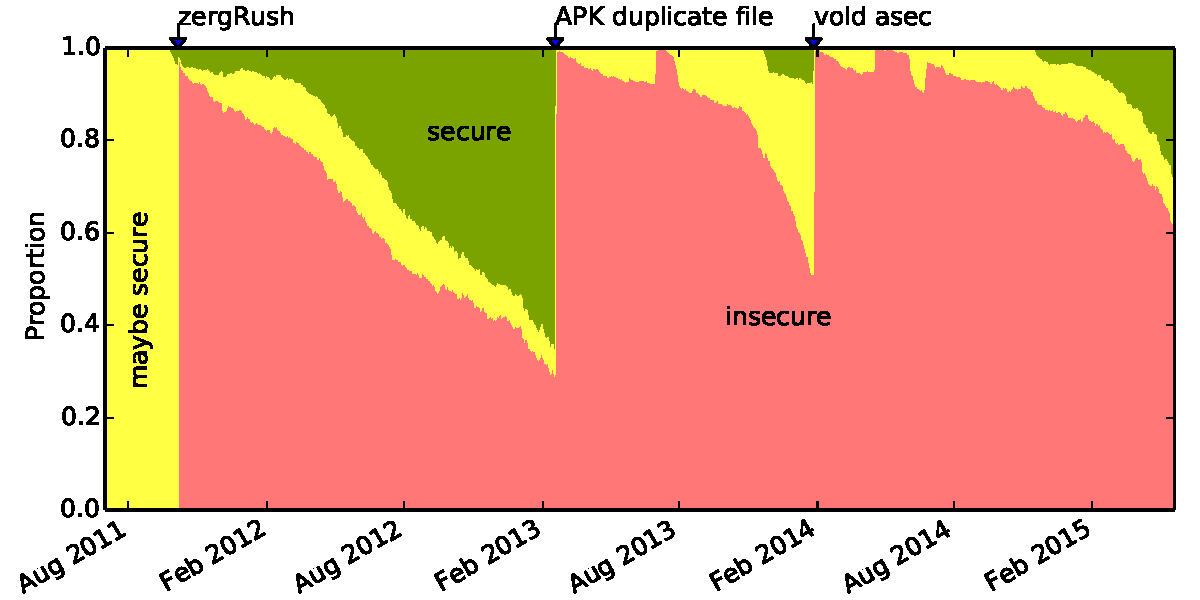
\includegraphics[width=\columnwidth]{figures/proportioninsecure}
%TODO make this graph shorter
\caption{Proportion of devices running insecure versions of android}
\label{fig:proportioninsecure}
\end{figure}

In the past users of Microsoft IIS were advised to switch to a different web server due to the high rate of vulnerability~\cite{Pescatore2001} this pressure helped cause Microsoft to focus on security so that it now does much better~\cite{TODO}.
Part of the reason why deployed devices do not receive updates in a timely manner is that there is little data on what is actually happening and so it is not possible to determine which manufacturers or operators are doing a better job.
Hence there is little incentive for manufacturers and operators to do a better job, we provide this data  in~\S\ref{sec:security_scoring} and discuss incentives further in \S\ref{sec:economics}

\section{Background}
\label{sec:background}
There are two sources of data we needed for this study, information on root exploits and information on installed versions of Android.

\subsection{Root exploits}
We compiled a list of root exploit vulnerabilities for Android containing information on when they were known about, what versions they affected and which versions fixed the problem.
We only looked for \emph{root equivalent} exploits which did not require USB debugging to exploit.
\emph{Root equivalent} means that it grants privileges equivalent in scope to root which can then be used to gain root.
Some phones can be `rooted' by enabling USB debugging and using the special privileges of the adb shell to root the device but only \daAdbPerc\ of devices have USB debugging enabled.
This is not something that applications running on the phone can exploit to break compartmentalisation and so we do not include those exploits.
Unfortunately many published exploits use adb for convenience and so determining whether that is necessary to exploit the vulnerability can be difficult.
Some exploits which grant root are not traditional kernel exploits, for example the discovery of flaws in the verification of signatures on Android applications in February 2013~\cite{Forristal2013} meant that applications could pretend to be signed with system keys and hence gain root privileges.

We have published full details of the \daNumVulnsUsed\ vulnerabilities used for this analysis in an accompanying technical report~\cite{TODO} and summarise them in Table \ref{tab:andvulns}.
We also have a website\footnote{\url{http://androidvulnerabilities.org/}} which we will keep up to date with future vulnerabilities and which has successfully solicited submissions from others.
In this analysis we only use vulnerabilities which affected all Android devices, not any of the manufacturer or hardware specific vulnerabilities

There was much manual effort required to track down details of these vulnerabilities as many of them are not in other databases such as the CVE database, the lack of a widely acknowledged unique identifier made identifying whether two reports referenced the same vulnerability difficult.
Previous work has assumed ``any security issue of relevance will eventually get a CVE number assigned"~\cite{Frei2010} which is currently not the case for Android with several root vulnerabilities not having CVE numbers.
For some of the vulnerabilities without CVE numbers we checked with Google whether they had one assigned and they confirmed that there was no number and that they did not intend to get one (though they did give us the Android bug number and tell us to use that).

Working out the date to use for the date on which a vulnerability was sufficiently well known to pose a threat to users is difficult.
Frei et al.\ propose the definition of the {\bf time of disclosure} when the information about the vulnerability is freely available to the public, from a widely accepted and independent source and has been validated by security experts so that it has a risk rating.
Unfortunately before we collated this information much of it was not published by an independent source and lacked risk rating information, even months or years after they had been actively used.

Prior work~\cite{Bilge2012} has shown that after public disclosure exploitation rates increase by 5 orders of magnitude and so from the point of view of widespread danger, the period between public disclosure and the update reaching the user's device is the most critical.
However they also show that zero day exploits are typically used for 312 days before they are publicly disclosed, often to target particular organisations.
Hence when considering vulnerability from the point of view of an organisation which cares about Advanced Persistent Threats, such as those the CESG advice~\cite{CESG2013} is aimed at, the critical period is from when people could have started using the vulnerability to when the update hits the user device.
So for our vulnerability calculations we use the earliest date we can find recorded evidence that the vulnerability was known about, even if that knowledge might have been confined to a particular manufacturer or hobbyist.
We cannot know if someone reported the vulnerability to the manufacturer and we do know that various agencies are engaged in widespread monitoring of communications and compromise of civilian infrastructure~\cite{TODO} and so they probably know.
Hence we use dates such as: when CVEs were registered, when fixes were committed to source repositories, or when exploits were committed to repositories; as the date first known about.

\daTabAndVulns

\subsection{Versions of Android running on devices}
We also need historical information on which versions of Android were running on devices along with other information about those devices which allows us to go into more detail and confirm the reliability of the data our results depend on.
The only suitable data which is available for this is the Device Analyzer data~\cite{Wagner2013}.
The Device Analyzer data contains data from \daNumDevices\ devices with a total of \daDeviceDays\ device days, it contains data for more than \daMonths months for \daMonthsDevices\ devices.
%TODO talk about the Device Analyzer project a bit
Various different kinds of data\footnote{\url{https://deviceanalyzer.cl.cam.ac.uk/collected.htm}} are collected by the Device Analyzer Android app\footnote{\url{https://deviceanalyzer.cl.cam.ac.uk/}}.
Among these are the build string and API version for the version of Android currently running on the device each day.
The API/SDK version is a well defined integer, however it does not always change with new Android releases, particularly security bug fixes should not increase this value.
The build string is `The user-visible version string', fortunately most (99.9\%) devices in the data have a build string of the form `x.y.z random string' and so it is possible to extract the Android version number.
On a large proportion of devices `random string' is a well defined build number but different manufacturers use different schema.

\subsection{Running a version of Android known to be vulnerable makes a device vulnerable}
While we have not tried to exploit these vulnerabilities on the devices in order to test whether the devices are actually vulnerable, we are confident that most devices will be if they are running a vesion known to be vulnerable.

\section{Results}
\label{sec:results}
In this section we present the results of our analysis showing \daMeanInsecurityPerc\ of devices to have root vulnerabilities on average, nexus devices to be better than others, \daSecScoreBestmanufacturer\ to be the best manufacturer and ????. %TODO summarise our results
%TODO comparison of nexus update rates with iOS


The proportion of devices in the Device Analyzer data running different versions of Android each day is shown in Figure~\ref{fig:norm_os}.
It shows how old versions are gradually replaced by new ones, the long tail of devices which do not see updates to more recent versions and the fluctuation in the number of devices in the data.
We verify the validity of this data in \S\ref{sec:representative}.
\begin{figure}
 \centering
 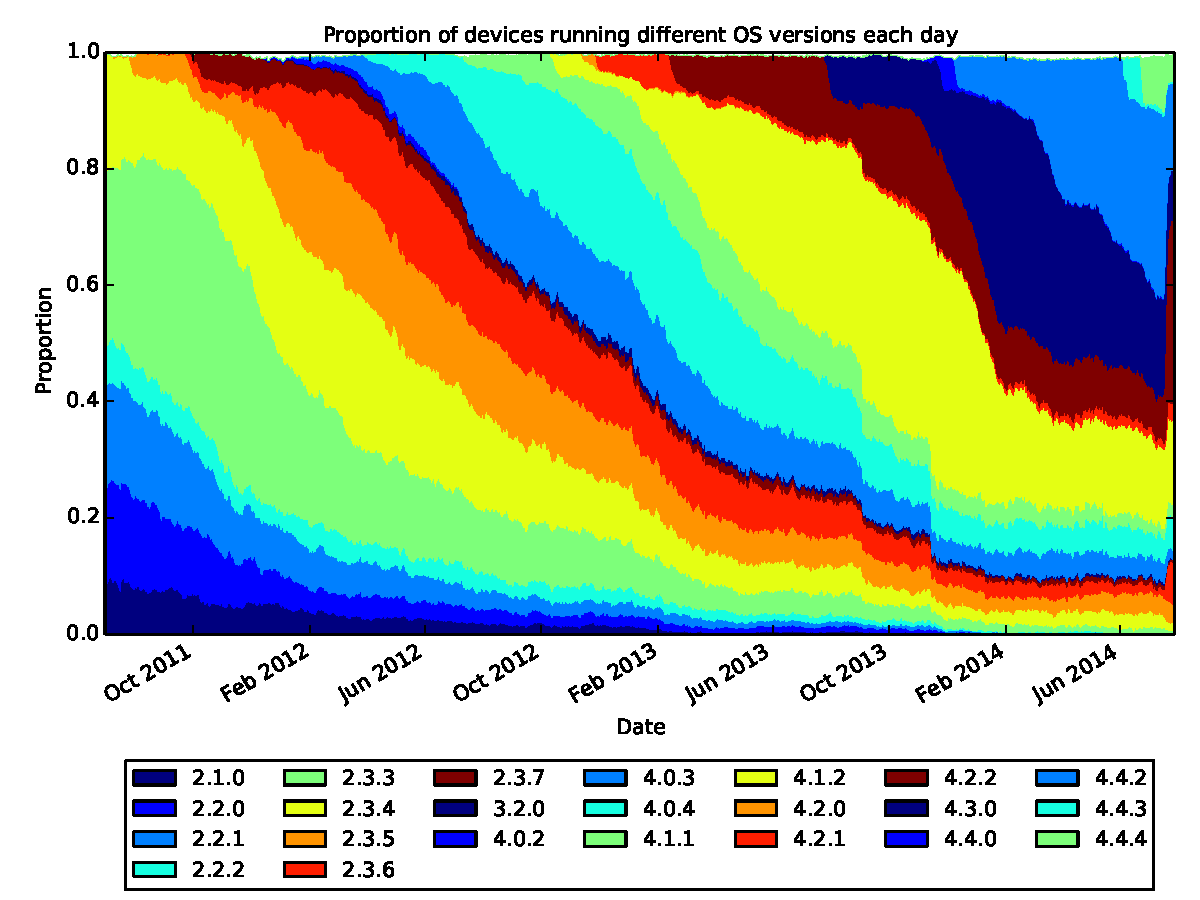
\includegraphics[width=\columnwidth]{figures/da_norm_os}
 \caption{Android versions in Device Analyzer data over time}
 \label{fig:norm_os}
\end{figure}

Figure \ref{fig:vulnerabilities} shows which vulnerabilities devices are exposed to.
For each vulnerability it shows the proportion of devices exposed to that vulnerability and how that changes over time.
In July 2011 at the beginning of the Device Analyzer data the Exploid and Levitator vulnerabilities both affect most Android devices, slowly these are fixed as updates roll out and devices are replaced until in January 2013 a much smaller proportion of devices are affected by known vulnerabilities.
However when in February 2013 the first APK signing vulnerability was found which affected all previous versions of Android and even in October 2013 most devices were still unfixed. %TODO put percentages on these things to quantify them
\begin{figure}%[!b]
\centering
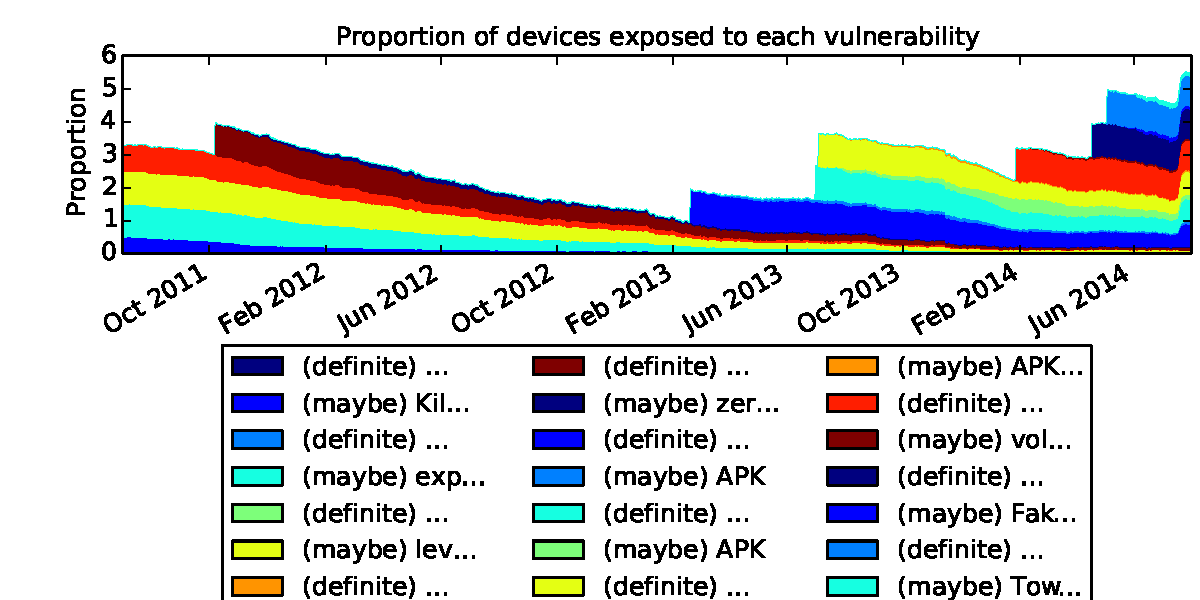
\includegraphics[width=\columnwidth]{figures/vulnerabilities}
\caption{Proportion of devices exposed to each vulnerability with time (1.0 is 100\%)}
\label{fig:vulnerabilities}
\end{figure}

The variation of the proportion of devices affected by a vulnerability with time tells us how bad a particular vulnerability affected the Android platform.
Figure \ref{fig:nvulnerabilities_heat} breaks this down by vulnerability to show how the proportion of devices affected by different vulnerabilities varies.
In 2013 three vulnerabilities were found in the way which Android verified the signatures on APKs.
These allowed the creation of malicious APKs which appear to be signed as system APKs -- which have root equivalent privileges.
Figure \ref{fig:nvulnerabilities_heat} shows how the the \emph{APK signing vulnerabilities} affected all devices and took months to get fixed for any device.
However what is perhaps more worrying is the long tail on the \emph{Gingerbreak}, \emph{levitator} and \emph{exploid} vulnerabilities which are more dangerous root exploits (not requiring new APK installation) and which still affect a significant proportion of devices years later.

\begin{figure}
 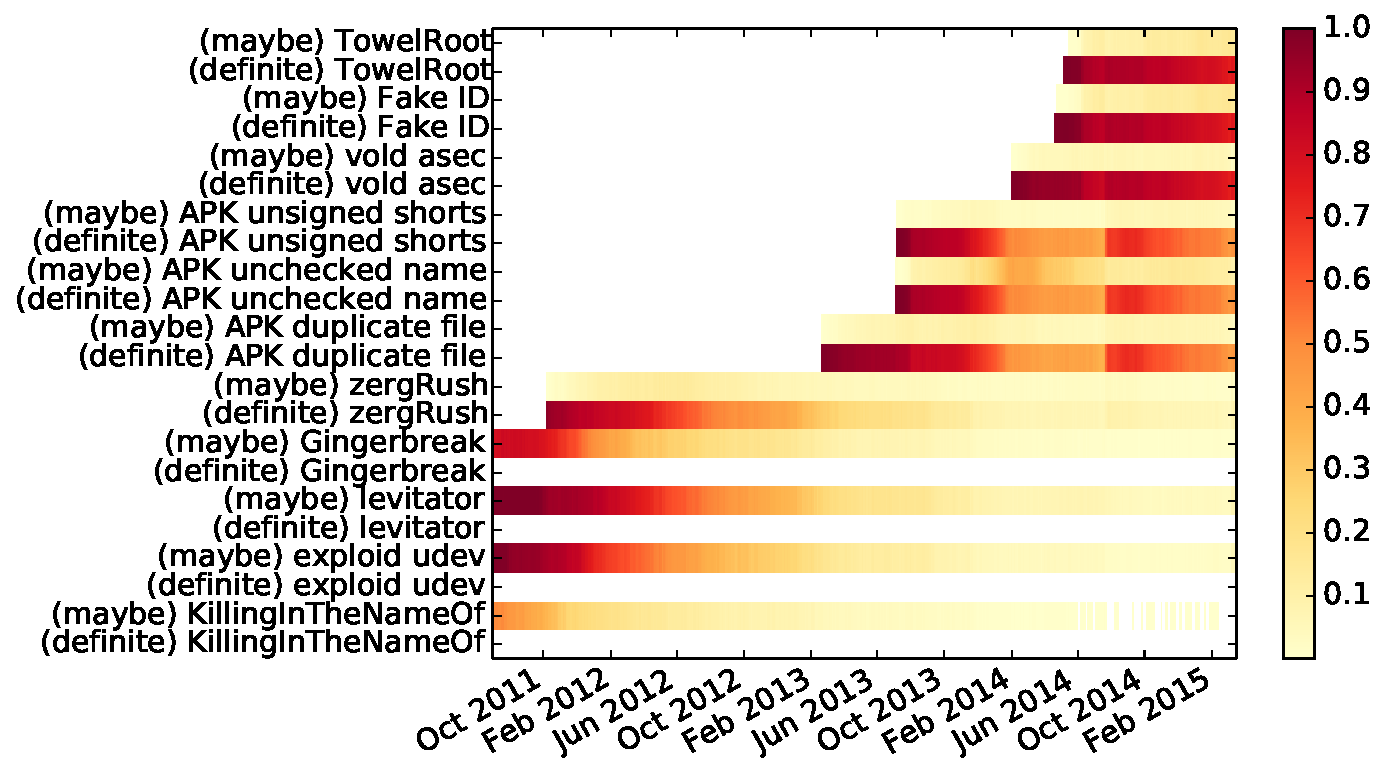
\includegraphics[width=0.5\textwidth]{figures/nvulnerabilities_heat.pdf}
 \caption{Proportion of devices affected by different vulnerabilities}
 \label{fig:nvulnerabilities_heat}
\end{figure}

\subsection{Update frequency}
%TODO find out what the frequency of updates is
\begin{figure}
 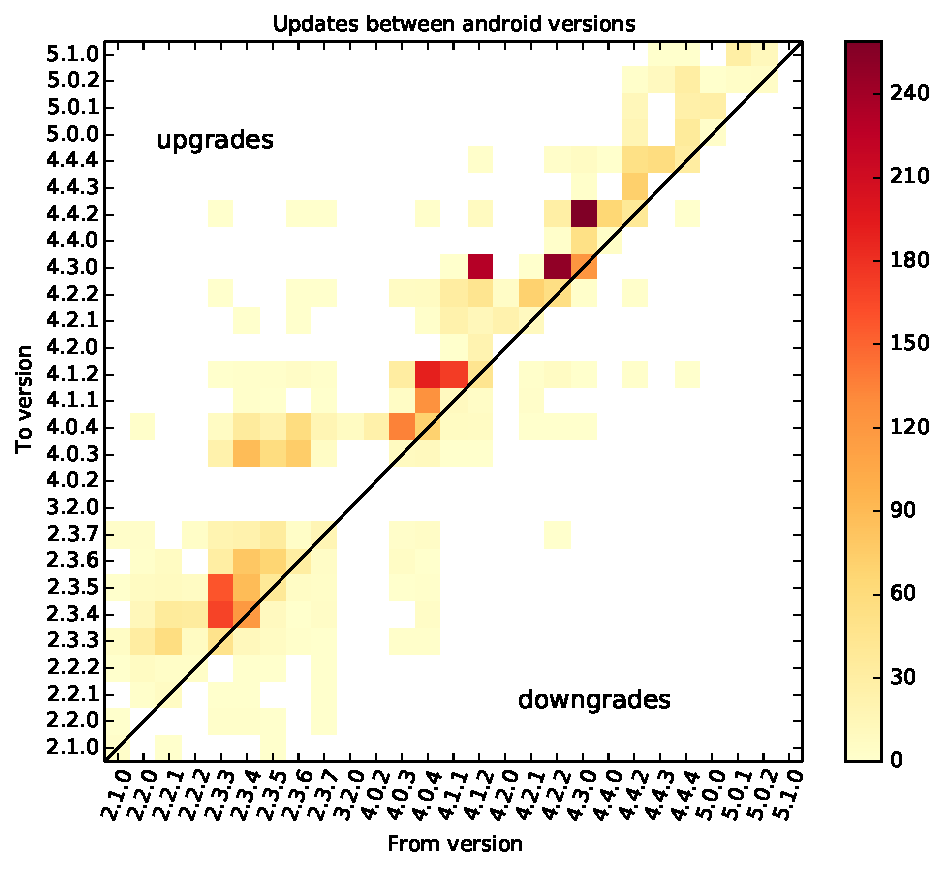
\includegraphics[width=0.5\textwidth]{figures/from_to_updates.pdf}
 \caption{Updates between different Android versions in the DA data}
 \label{fig:from_to_updates}
\end{figure}
\begin{figure}
 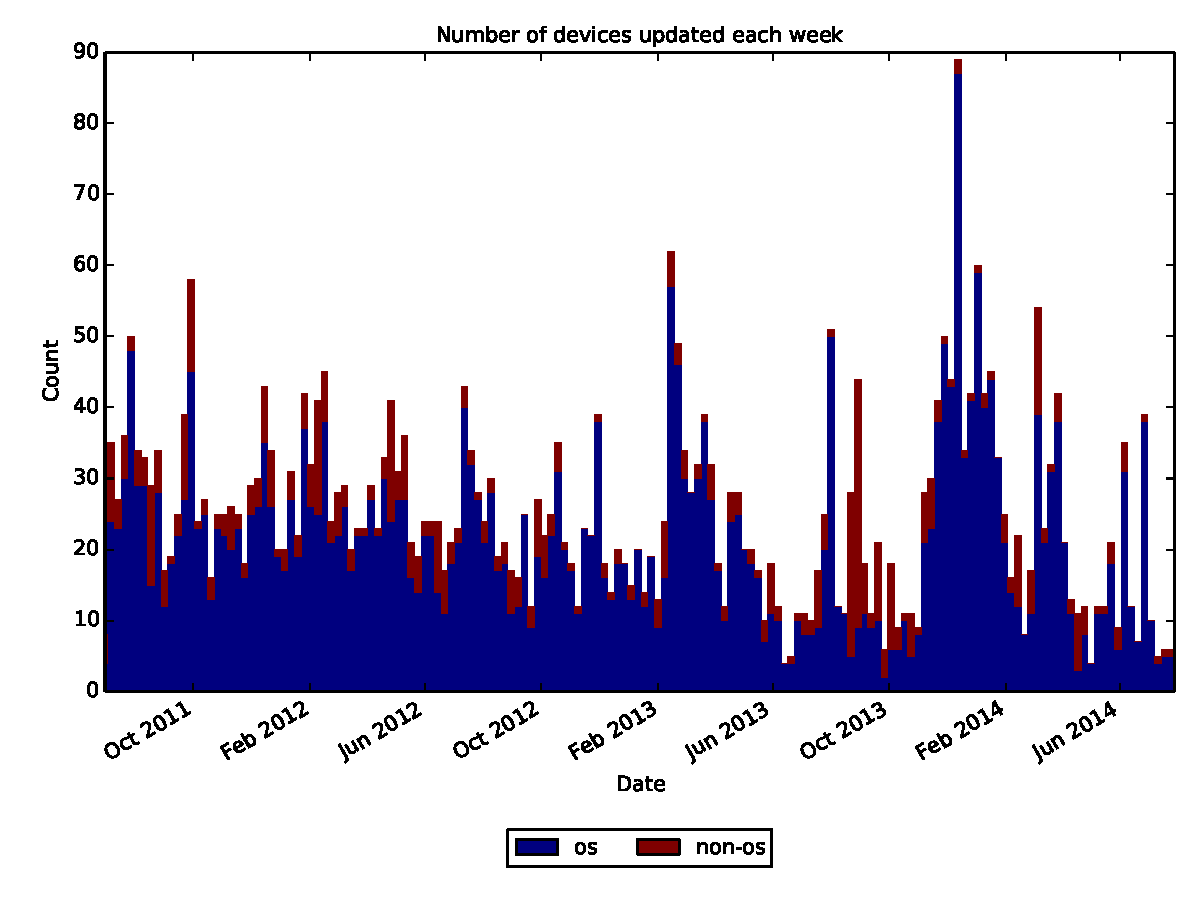
\includegraphics[width=0.5\textwidth]{figures/w_security_updates.pdf}
 \caption{Number of updates each week which fixed or may have fixed security vulnerabilities}
 \label{fig:weekly_security_updates}
\end{figure}
Figure \ref{fig:from_to_updates} shows how devices upgrade between different versions of Android.
Device Analyzer (DA) observes upgrade events and the figure shows which versions a device is upgrading from and to.
Mostly the dark cells are above the diagonal and are upgrades.
While many upgrades are from one version to the next version there are also a fair number which skip a few versions.
Surprisingly there are also a small number of downgrade events when older versions of Android are installed on to devices.
The number of devices getting security updates each week, is shown in Figure \ref{fig:weekly_security_updates}, blue shows updates which changed the Android version number from a version with known vulnerabilities to one which had fewer known vulnerabilities.
Red indicates updates which changed the build number but not the version number and so might contain a backported fix for a vulnerability.
%TODO summary stats, what does this mean


\section{Comparing device manufacturers, device models and network operators}
\label{sec:security_scoring}\label{sec:exp:security_score}

To allow buyers of Android devices to purchase those devices which have the best security they need to know how different device manufacturers, device models and network operators compare in terms of the security they provide.
We propose a method to score a device manufacturer, device model or network operator based on its historic performance at keeping devices up-to-date and fixing security vulnerabilities.
We find that Android as a whole gets a score of \daSecurityScore\ out of 10, the highest scoring device manufacturer is \emph{\daSecScoreBestmanufacturer} (\daSecScoreBestmanufacturerScore\ out of 10) and the lowest scoring is \emph{\daSecScoreWorstmanufacturer} (\daSecScoreWorstmanufacturerScore\ out of 10).

\subsection{Method: Scoring for security}\label{sec:security_scoring:method}

Computing how good a particular device manufacturer or device model is from a security standpoint is difficult as it depends on a number of factors which are hard to observe, particularly on a large scale.
Ideally we would consider both the prevalence of potential problems which were not exploited and actual security failures.
%\footnote{A perfectly secure operating system would among other things detect and prevent all phishing attacks, provide perfect principle of least privilege isolation, not have any vulnerabilities, instantly fix all discovered vulnerabilities, not allow any user data to be used in a way which the user does not approve of and be really easy for an ordinary person to use.}
However in the absence of such data we propose a scheme for assigning a device a score out of ten based on data which can be observed, is based on previous metrics, and which we expect correlates with the actual security of the devices.

The FUM score is computed from three components:
\begin{description}
  \item[free $f$] The proportion of running devices which were free from critical vulnerabilities over time. This is equivalent to Acer and Jackson's proposal to measure the security based on the proportion of users with at least one unpatched critical vulnerability~\cite{Acer2010} and similar to the Vulnerability Free Days (VFD) score~\cite{Wright2014}.
  Unlike VFD this is the proportion of running devices which were free from critical vulnerabilities over time, rather than days which the device manufacturer was free from outstanding critical vulnerabilities as that does not take account of the update process.
  \item[update $u$] The proportion of devices which run the latest version of Android shipped to any device produced by that device manufacturer. This is a measure of internal updatedness, a low score would mean many devices are being left behind.
  This assumes that newer versions are better with stronger security.
  Historically steps have been taken to improve Android security in newer versions so this assumption should generally hold, but sometimes new updates introduce new vulnerabilities.
  \item[mean $m$] The mean number of outstanding vulnerabilities affecting devices not fixed on any device shipped by the device manufacturer. This is related to the Median Active Vulnerabilities (MAV) measure~\cite{Wright2014} but is the mean rather than the median, as this gives a continuous value.
  An example is given in Figure~\ref{fig:mcalculation}.
%TODO should we compute the median instead?
\end{description}

\begin{figure}
\centering
%\includegraphics[width=\columnwidth]{figures/mcalculation}
% Graphic for TeX using PGF
% Title: /home/drt24/git/papers/da/securityupdates/figures/mcalculation.dia
% Creator: Dia v0.97.3
% CreationDate: Wed Apr 22 15:03:07 2015
% For: drt24
% \usepackage{tikz}
% The following commands are not supported in PSTricks at present
% We define them conditionally, so when they are implemented,
% this pgf file will use them.
\ifx\du\undefined
  \newlength{\du}
\fi
\setlength{\du}{5\unitlength}
\begin{tikzpicture}
\pgftransformxscale{1.000000}
\pgftransformyscale{-1.000000}
\definecolor{dialinecolor}{rgb}{0.000000, 0.000000, 0.000000}
\pgfsetstrokecolor{dialinecolor}
\definecolor{dialinecolor}{rgb}{1.000000, 1.000000, 1.000000}
\pgfsetfillcolor{dialinecolor}
\pgfsetlinewidth{0.100000\du}
\pgfsetdash{{\pgflinewidth}{0.200000\du}}{0cm}
\pgfsetdash{{\pgflinewidth}{0.200000\du}}{0cm}
\pgfsetbuttcap
{
\definecolor{dialinecolor}{rgb}{0.000000, 0.000000, 0.000000}
\pgfsetfillcolor{dialinecolor}
% was here!!!
\definecolor{dialinecolor}{rgb}{0.000000, 0.000000, 0.000000}
\pgfsetstrokecolor{dialinecolor}
\draw (5.000000\du,24.000000\du)--(5.000000\du,9.000000\du);
}
\pgfsetlinewidth{0.100000\du}
\pgfsetdash{{\pgflinewidth}{0.200000\du}}{0cm}
\pgfsetdash{{\pgflinewidth}{0.200000\du}}{0cm}
\pgfsetbuttcap
{
\definecolor{dialinecolor}{rgb}{0.000000, 0.000000, 0.000000}
\pgfsetfillcolor{dialinecolor}
% was here!!!
\definecolor{dialinecolor}{rgb}{0.000000, 0.000000, 0.000000}
\pgfsetstrokecolor{dialinecolor}
\draw (7.000000\du,24.000000\du)--(7.000000\du,9.000000\du);
}
\pgfsetlinewidth{0.100000\du}
\pgfsetdash{{\pgflinewidth}{0.200000\du}}{0cm}
\pgfsetdash{{\pgflinewidth}{0.200000\du}}{0cm}
\pgfsetbuttcap
{
\definecolor{dialinecolor}{rgb}{0.000000, 0.000000, 0.000000}
\pgfsetfillcolor{dialinecolor}
% was here!!!
\definecolor{dialinecolor}{rgb}{0.000000, 0.000000, 0.000000}
\pgfsetstrokecolor{dialinecolor}
\draw (9.000000\du,24.000000\du)--(9.000000\du,9.000000\du);
}
\pgfsetlinewidth{0.100000\du}
\pgfsetdash{{\pgflinewidth}{0.200000\du}}{0cm}
\pgfsetdash{{\pgflinewidth}{0.200000\du}}{0cm}
\pgfsetbuttcap
{
\definecolor{dialinecolor}{rgb}{0.000000, 0.000000, 0.000000}
\pgfsetfillcolor{dialinecolor}
% was here!!!
\definecolor{dialinecolor}{rgb}{0.000000, 0.000000, 0.000000}
\pgfsetstrokecolor{dialinecolor}
\draw (11.000000\du,24.000000\du)--(11.000000\du,9.000000\du);
}
\pgfsetlinewidth{0.100000\du}
\pgfsetdash{{\pgflinewidth}{0.200000\du}}{0cm}
\pgfsetdash{{\pgflinewidth}{0.200000\du}}{0cm}
\pgfsetbuttcap
{
\definecolor{dialinecolor}{rgb}{0.000000, 0.000000, 0.000000}
\pgfsetfillcolor{dialinecolor}
% was here!!!
\definecolor{dialinecolor}{rgb}{0.000000, 0.000000, 0.000000}
\pgfsetstrokecolor{dialinecolor}
\draw (13.000000\du,24.000000\du)--(13.000000\du,9.000000\du);
}
\pgfsetlinewidth{0.100000\du}
\pgfsetdash{{\pgflinewidth}{0.200000\du}}{0cm}
\pgfsetdash{{\pgflinewidth}{0.200000\du}}{0cm}
\pgfsetbuttcap
{
\definecolor{dialinecolor}{rgb}{0.000000, 0.000000, 0.000000}
\pgfsetfillcolor{dialinecolor}
% was here!!!
\definecolor{dialinecolor}{rgb}{0.000000, 0.000000, 0.000000}
\pgfsetstrokecolor{dialinecolor}
\draw (15.000000\du,24.000000\du)--(15.000000\du,9.000000\du);
}
\pgfsetlinewidth{0.100000\du}
\pgfsetdash{{\pgflinewidth}{0.200000\du}}{0cm}
\pgfsetdash{{\pgflinewidth}{0.200000\du}}{0cm}
\pgfsetbuttcap
{
\definecolor{dialinecolor}{rgb}{0.000000, 0.000000, 0.000000}
\pgfsetfillcolor{dialinecolor}
% was here!!!
\definecolor{dialinecolor}{rgb}{0.000000, 0.000000, 0.000000}
\pgfsetstrokecolor{dialinecolor}
\draw (17.000000\du,24.000000\du)--(17.000000\du,9.000000\du);
}
\pgfsetlinewidth{0.100000\du}
\pgfsetdash{{\pgflinewidth}{0.200000\du}}{0cm}
\pgfsetdash{{\pgflinewidth}{0.200000\du}}{0cm}
\pgfsetbuttcap
{
\definecolor{dialinecolor}{rgb}{0.000000, 0.000000, 0.000000}
\pgfsetfillcolor{dialinecolor}
% was here!!!
\definecolor{dialinecolor}{rgb}{0.000000, 0.000000, 0.000000}
\pgfsetstrokecolor{dialinecolor}
\draw (19.000000\du,24.000000\du)--(19.000000\du,9.000000\du);
}
\pgfsetlinewidth{0.100000\du}
\pgfsetdash{{\pgflinewidth}{0.200000\du}}{0cm}
\pgfsetdash{{\pgflinewidth}{0.200000\du}}{0cm}
\pgfsetbuttcap
{
\definecolor{dialinecolor}{rgb}{0.000000, 0.000000, 0.000000}
\pgfsetfillcolor{dialinecolor}
% was here!!!
\definecolor{dialinecolor}{rgb}{0.000000, 0.000000, 0.000000}
\pgfsetstrokecolor{dialinecolor}
\draw (21.000000\du,24.000000\du)--(21.000000\du,9.000000\du);
}
\pgfsetlinewidth{0.100000\du}
\pgfsetdash{{\pgflinewidth}{0.200000\du}}{0cm}
\pgfsetdash{{\pgflinewidth}{0.200000\du}}{0cm}
\pgfsetbuttcap
{
\definecolor{dialinecolor}{rgb}{0.000000, 0.000000, 0.000000}
\pgfsetfillcolor{dialinecolor}
% was here!!!
\definecolor{dialinecolor}{rgb}{0.000000, 0.000000, 0.000000}
\pgfsetstrokecolor{dialinecolor}
\draw (23.000000\du,24.000000\du)--(23.000000\du,9.000000\du);
}
\pgfsetlinewidth{0.100000\du}
\pgfsetdash{{\pgflinewidth}{0.200000\du}}{0cm}
\pgfsetdash{{\pgflinewidth}{0.200000\du}}{0cm}
\pgfsetbuttcap
{
\definecolor{dialinecolor}{rgb}{0.000000, 0.000000, 0.000000}
\pgfsetfillcolor{dialinecolor}
% was here!!!
\definecolor{dialinecolor}{rgb}{0.000000, 0.000000, 0.000000}
\pgfsetstrokecolor{dialinecolor}
\draw (25.000000\du,24.000000\du)--(25.000000\du,9.000000\du);
}
\pgfsetlinewidth{0.100000\du}
\pgfsetdash{{\pgflinewidth}{0.200000\du}}{0cm}
\pgfsetdash{{\pgflinewidth}{0.200000\du}}{0cm}
\pgfsetbuttcap
{
\definecolor{dialinecolor}{rgb}{0.000000, 0.000000, 0.000000}
\pgfsetfillcolor{dialinecolor}
% was here!!!
\definecolor{dialinecolor}{rgb}{0.000000, 0.000000, 0.000000}
\pgfsetstrokecolor{dialinecolor}
\draw (27.000000\du,24.000000\du)--(27.000000\du,9.000000\du);
}
\pgfsetlinewidth{0.100000\du}
\pgfsetdash{{\pgflinewidth}{0.200000\du}}{0cm}
\pgfsetdash{{\pgflinewidth}{0.200000\du}}{0cm}
\pgfsetbuttcap
{
\definecolor{dialinecolor}{rgb}{0.000000, 0.000000, 0.000000}
\pgfsetfillcolor{dialinecolor}
% was here!!!
\definecolor{dialinecolor}{rgb}{0.000000, 0.000000, 0.000000}
\pgfsetstrokecolor{dialinecolor}
\draw (29.000000\du,24.000000\du)--(29.000000\du,9.000000\du);
}
\pgfsetlinewidth{0.100000\du}
\pgfsetdash{{\pgflinewidth}{0.200000\du}}{0cm}
\pgfsetdash{{\pgflinewidth}{0.200000\du}}{0cm}
\pgfsetbuttcap
{
\definecolor{dialinecolor}{rgb}{0.000000, 0.000000, 0.000000}
\pgfsetfillcolor{dialinecolor}
% was here!!!
\definecolor{dialinecolor}{rgb}{0.000000, 0.000000, 0.000000}
\pgfsetstrokecolor{dialinecolor}
\draw (31.000000\du,24.000000\du)--(31.000000\du,9.000000\du);
}
\pgfsetlinewidth{0.100000\du}
\pgfsetdash{}{0pt}
\pgfsetdash{}{0pt}
\pgfsetbuttcap
{
\definecolor{dialinecolor}{rgb}{0.000000, 0.000000, 0.000000}
\pgfsetfillcolor{dialinecolor}
% was here!!!
\pgfsetarrowsend{latex}
\definecolor{dialinecolor}{rgb}{0.000000, 0.000000, 0.000000}
\pgfsetstrokecolor{dialinecolor}
\draw (5.000000\du,24.000000\du)--(46.000000\du,24.000000\du);
}
\pgfsetlinewidth{0.100000\du}
\pgfsetdash{}{0pt}
\pgfsetdash{}{0pt}
\pgfsetbuttcap
{
\definecolor{dialinecolor}{rgb}{0.000000, 0.000000, 0.000000}
\pgfsetfillcolor{dialinecolor}
% was here!!!
}
\definecolor{dialinecolor}{rgb}{0.000000, 0.000000, 0.000000}
\pgfsetstrokecolor{dialinecolor}
\draw (7.250000\du,13.000000\du)--(25.300000\du,13.000000\du);
\pgfsetlinewidth{0.100000\du}
\pgfsetdash{}{0pt}
\pgfsetmiterjoin
\pgfsetbuttcap
\definecolor{dialinecolor}{rgb}{1.000000, 1.000000, 1.000000}
\pgfsetfillcolor{dialinecolor}
\pgfpathmoveto{\pgfpoint{6.750000\du}{13.000000\du}}
\pgfpathcurveto{\pgfpoint{6.750000\du}{12.875000\du}}{\pgfpoint{6.875000\du}{12.750000\du}}{\pgfpoint{7.000000\du}{12.750000\du}}
\pgfpathcurveto{\pgfpoint{7.125000\du}{12.750000\du}}{\pgfpoint{7.250000\du}{12.875000\du}}{\pgfpoint{7.250000\du}{13.000000\du}}
\pgfpathcurveto{\pgfpoint{7.250000\du}{13.125000\du}}{\pgfpoint{7.125000\du}{13.250000\du}}{\pgfpoint{7.000000\du}{13.250000\du}}
\pgfpathcurveto{\pgfpoint{6.875000\du}{13.250000\du}}{\pgfpoint{6.750000\du}{13.125000\du}}{\pgfpoint{6.750000\du}{13.000000\du}}
\pgfusepath{fill}
\definecolor{dialinecolor}{rgb}{0.000000, 0.000000, 0.000000}
\pgfsetstrokecolor{dialinecolor}
\pgfpathmoveto{\pgfpoint{6.750000\du}{13.000000\du}}
\pgfpathcurveto{\pgfpoint{6.750000\du}{12.875000\du}}{\pgfpoint{6.875000\du}{12.750000\du}}{\pgfpoint{7.000000\du}{12.750000\du}}
\pgfpathcurveto{\pgfpoint{7.125000\du}{12.750000\du}}{\pgfpoint{7.250000\du}{12.875000\du}}{\pgfpoint{7.250000\du}{13.000000\du}}
\pgfpathcurveto{\pgfpoint{7.250000\du}{13.125000\du}}{\pgfpoint{7.125000\du}{13.250000\du}}{\pgfpoint{7.000000\du}{13.250000\du}}
\pgfpathcurveto{\pgfpoint{6.875000\du}{13.250000\du}}{\pgfpoint{6.750000\du}{13.125000\du}}{\pgfpoint{6.750000\du}{13.000000\du}}
\pgfusepath{stroke}
\pgfsetlinewidth{0.100000\du}
\pgfsetdash{}{0pt}
\pgfsetmiterjoin
\pgfsetbuttcap
\definecolor{dialinecolor}{rgb}{0.000000, 0.000000, 0.000000}
\pgfsetfillcolor{dialinecolor}
\pgfpathmoveto{\pgfpoint{25.300000\du}{13.000000\du}}
\pgfpathcurveto{\pgfpoint{25.300000\du}{13.125000\du}}{\pgfpoint{25.175000\du}{13.250000\du}}{\pgfpoint{25.050000\du}{13.250000\du}}
\pgfpathcurveto{\pgfpoint{24.925000\du}{13.250000\du}}{\pgfpoint{24.800000\du}{13.125000\du}}{\pgfpoint{24.800000\du}{13.000000\du}}
\pgfpathcurveto{\pgfpoint{24.800000\du}{12.875000\du}}{\pgfpoint{24.925000\du}{12.750000\du}}{\pgfpoint{25.050000\du}{12.750000\du}}
\pgfpathcurveto{\pgfpoint{25.175000\du}{12.750000\du}}{\pgfpoint{25.300000\du}{12.875000\du}}{\pgfpoint{25.300000\du}{13.000000\du}}
\pgfusepath{fill}
\definecolor{dialinecolor}{rgb}{0.000000, 0.000000, 0.000000}
\pgfsetstrokecolor{dialinecolor}
\pgfpathmoveto{\pgfpoint{25.300000\du}{13.000000\du}}
\pgfpathcurveto{\pgfpoint{25.300000\du}{13.125000\du}}{\pgfpoint{25.175000\du}{13.250000\du}}{\pgfpoint{25.050000\du}{13.250000\du}}
\pgfpathcurveto{\pgfpoint{24.925000\du}{13.250000\du}}{\pgfpoint{24.800000\du}{13.125000\du}}{\pgfpoint{24.800000\du}{13.000000\du}}
\pgfpathcurveto{\pgfpoint{24.800000\du}{12.875000\du}}{\pgfpoint{24.925000\du}{12.750000\du}}{\pgfpoint{25.050000\du}{12.750000\du}}
\pgfpathcurveto{\pgfpoint{25.175000\du}{12.750000\du}}{\pgfpoint{25.300000\du}{12.875000\du}}{\pgfpoint{25.300000\du}{13.000000\du}}
\pgfusepath{stroke}
\pgfsetlinewidth{0.100000\du}
\pgfsetdash{}{0pt}
\pgfsetdash{}{0pt}
\pgfsetbuttcap
{
\definecolor{dialinecolor}{rgb}{0.000000, 0.000000, 0.000000}
\pgfsetfillcolor{dialinecolor}
% was here!!!
}
\definecolor{dialinecolor}{rgb}{0.000000, 0.000000, 0.000000}
\pgfsetstrokecolor{dialinecolor}
\draw (9.250000\du,11.000000\du)--(15.300000\du,11.000000\du);
\pgfsetlinewidth{0.100000\du}
\pgfsetdash{}{0pt}
\pgfsetmiterjoin
\pgfsetbuttcap
\definecolor{dialinecolor}{rgb}{1.000000, 1.000000, 1.000000}
\pgfsetfillcolor{dialinecolor}
\pgfpathmoveto{\pgfpoint{8.750000\du}{11.000000\du}}
\pgfpathcurveto{\pgfpoint{8.750000\du}{10.875000\du}}{\pgfpoint{8.875000\du}{10.750000\du}}{\pgfpoint{9.000000\du}{10.750000\du}}
\pgfpathcurveto{\pgfpoint{9.125000\du}{10.750000\du}}{\pgfpoint{9.250000\du}{10.875000\du}}{\pgfpoint{9.250000\du}{11.000000\du}}
\pgfpathcurveto{\pgfpoint{9.250000\du}{11.125000\du}}{\pgfpoint{9.125000\du}{11.250000\du}}{\pgfpoint{9.000000\du}{11.250000\du}}
\pgfpathcurveto{\pgfpoint{8.875000\du}{11.250000\du}}{\pgfpoint{8.750000\du}{11.125000\du}}{\pgfpoint{8.750000\du}{11.000000\du}}
\pgfusepath{fill}
\definecolor{dialinecolor}{rgb}{0.000000, 0.000000, 0.000000}
\pgfsetstrokecolor{dialinecolor}
\pgfpathmoveto{\pgfpoint{8.750000\du}{11.000000\du}}
\pgfpathcurveto{\pgfpoint{8.750000\du}{10.875000\du}}{\pgfpoint{8.875000\du}{10.750000\du}}{\pgfpoint{9.000000\du}{10.750000\du}}
\pgfpathcurveto{\pgfpoint{9.125000\du}{10.750000\du}}{\pgfpoint{9.250000\du}{10.875000\du}}{\pgfpoint{9.250000\du}{11.000000\du}}
\pgfpathcurveto{\pgfpoint{9.250000\du}{11.125000\du}}{\pgfpoint{9.125000\du}{11.250000\du}}{\pgfpoint{9.000000\du}{11.250000\du}}
\pgfpathcurveto{\pgfpoint{8.875000\du}{11.250000\du}}{\pgfpoint{8.750000\du}{11.125000\du}}{\pgfpoint{8.750000\du}{11.000000\du}}
\pgfusepath{stroke}
\pgfsetlinewidth{0.100000\du}
\pgfsetdash{}{0pt}
\pgfsetmiterjoin
\pgfsetbuttcap
\definecolor{dialinecolor}{rgb}{0.000000, 0.000000, 0.000000}
\pgfsetfillcolor{dialinecolor}
\pgfpathmoveto{\pgfpoint{15.300000\du}{11.000000\du}}
\pgfpathcurveto{\pgfpoint{15.300000\du}{11.125000\du}}{\pgfpoint{15.175000\du}{11.250000\du}}{\pgfpoint{15.050000\du}{11.250000\du}}
\pgfpathcurveto{\pgfpoint{14.925000\du}{11.250000\du}}{\pgfpoint{14.800000\du}{11.125000\du}}{\pgfpoint{14.800000\du}{11.000000\du}}
\pgfpathcurveto{\pgfpoint{14.800000\du}{10.875000\du}}{\pgfpoint{14.925000\du}{10.750000\du}}{\pgfpoint{15.050000\du}{10.750000\du}}
\pgfpathcurveto{\pgfpoint{15.175000\du}{10.750000\du}}{\pgfpoint{15.300000\du}{10.875000\du}}{\pgfpoint{15.300000\du}{11.000000\du}}
\pgfusepath{fill}
\definecolor{dialinecolor}{rgb}{0.000000, 0.000000, 0.000000}
\pgfsetstrokecolor{dialinecolor}
\pgfpathmoveto{\pgfpoint{15.300000\du}{11.000000\du}}
\pgfpathcurveto{\pgfpoint{15.300000\du}{11.125000\du}}{\pgfpoint{15.175000\du}{11.250000\du}}{\pgfpoint{15.050000\du}{11.250000\du}}
\pgfpathcurveto{\pgfpoint{14.925000\du}{11.250000\du}}{\pgfpoint{14.800000\du}{11.125000\du}}{\pgfpoint{14.800000\du}{11.000000\du}}
\pgfpathcurveto{\pgfpoint{14.800000\du}{10.875000\du}}{\pgfpoint{14.925000\du}{10.750000\du}}{\pgfpoint{15.050000\du}{10.750000\du}}
\pgfpathcurveto{\pgfpoint{15.175000\du}{10.750000\du}}{\pgfpoint{15.300000\du}{10.875000\du}}{\pgfpoint{15.300000\du}{11.000000\du}}
\pgfusepath{stroke}
\pgfsetlinewidth{0.100000\du}
\pgfsetdash{}{0pt}
\pgfsetdash{}{0pt}
\pgfsetbuttcap
{
\definecolor{dialinecolor}{rgb}{0.000000, 0.000000, 0.000000}
\pgfsetfillcolor{dialinecolor}
% was here!!!
}
\definecolor{dialinecolor}{rgb}{0.000000, 0.000000, 0.000000}
\pgfsetstrokecolor{dialinecolor}
\draw (13.250000\du,9.000000\du)--(21.300000\du,9.000000\du);
\pgfsetlinewidth{0.100000\du}
\pgfsetdash{}{0pt}
\pgfsetmiterjoin
\pgfsetbuttcap
\definecolor{dialinecolor}{rgb}{1.000000, 1.000000, 1.000000}
\pgfsetfillcolor{dialinecolor}
\pgfpathmoveto{\pgfpoint{12.750000\du}{9.000000\du}}
\pgfpathcurveto{\pgfpoint{12.750000\du}{8.875000\du}}{\pgfpoint{12.875000\du}{8.750000\du}}{\pgfpoint{13.000000\du}{8.750000\du}}
\pgfpathcurveto{\pgfpoint{13.125000\du}{8.750000\du}}{\pgfpoint{13.250000\du}{8.875000\du}}{\pgfpoint{13.250000\du}{9.000000\du}}
\pgfpathcurveto{\pgfpoint{13.250000\du}{9.125000\du}}{\pgfpoint{13.125000\du}{9.250000\du}}{\pgfpoint{13.000000\du}{9.250000\du}}
\pgfpathcurveto{\pgfpoint{12.875000\du}{9.250000\du}}{\pgfpoint{12.750000\du}{9.125000\du}}{\pgfpoint{12.750000\du}{9.000000\du}}
\pgfusepath{fill}
\definecolor{dialinecolor}{rgb}{0.000000, 0.000000, 0.000000}
\pgfsetstrokecolor{dialinecolor}
\pgfpathmoveto{\pgfpoint{12.750000\du}{9.000000\du}}
\pgfpathcurveto{\pgfpoint{12.750000\du}{8.875000\du}}{\pgfpoint{12.875000\du}{8.750000\du}}{\pgfpoint{13.000000\du}{8.750000\du}}
\pgfpathcurveto{\pgfpoint{13.125000\du}{8.750000\du}}{\pgfpoint{13.250000\du}{8.875000\du}}{\pgfpoint{13.250000\du}{9.000000\du}}
\pgfpathcurveto{\pgfpoint{13.250000\du}{9.125000\du}}{\pgfpoint{13.125000\du}{9.250000\du}}{\pgfpoint{13.000000\du}{9.250000\du}}
\pgfpathcurveto{\pgfpoint{12.875000\du}{9.250000\du}}{\pgfpoint{12.750000\du}{9.125000\du}}{\pgfpoint{12.750000\du}{9.000000\du}}
\pgfusepath{stroke}
\pgfsetlinewidth{0.100000\du}
\pgfsetdash{}{0pt}
\pgfsetmiterjoin
\pgfsetbuttcap
\definecolor{dialinecolor}{rgb}{0.000000, 0.000000, 0.000000}
\pgfsetfillcolor{dialinecolor}
\pgfpathmoveto{\pgfpoint{21.300000\du}{9.000000\du}}
\pgfpathcurveto{\pgfpoint{21.300000\du}{9.125000\du}}{\pgfpoint{21.175000\du}{9.250000\du}}{\pgfpoint{21.050000\du}{9.250000\du}}
\pgfpathcurveto{\pgfpoint{20.925000\du}{9.250000\du}}{\pgfpoint{20.800000\du}{9.125000\du}}{\pgfpoint{20.800000\du}{9.000000\du}}
\pgfpathcurveto{\pgfpoint{20.800000\du}{8.875000\du}}{\pgfpoint{20.925000\du}{8.750000\du}}{\pgfpoint{21.050000\du}{8.750000\du}}
\pgfpathcurveto{\pgfpoint{21.175000\du}{8.750000\du}}{\pgfpoint{21.300000\du}{8.875000\du}}{\pgfpoint{21.300000\du}{9.000000\du}}
\pgfusepath{fill}
\definecolor{dialinecolor}{rgb}{0.000000, 0.000000, 0.000000}
\pgfsetstrokecolor{dialinecolor}
\pgfpathmoveto{\pgfpoint{21.300000\du}{9.000000\du}}
\pgfpathcurveto{\pgfpoint{21.300000\du}{9.125000\du}}{\pgfpoint{21.175000\du}{9.250000\du}}{\pgfpoint{21.050000\du}{9.250000\du}}
\pgfpathcurveto{\pgfpoint{20.925000\du}{9.250000\du}}{\pgfpoint{20.800000\du}{9.125000\du}}{\pgfpoint{20.800000\du}{9.000000\du}}
\pgfpathcurveto{\pgfpoint{20.800000\du}{8.875000\du}}{\pgfpoint{20.925000\du}{8.750000\du}}{\pgfpoint{21.050000\du}{8.750000\du}}
\pgfpathcurveto{\pgfpoint{21.175000\du}{8.750000\du}}{\pgfpoint{21.300000\du}{8.875000\du}}{\pgfpoint{21.300000\du}{9.000000\du}}
\pgfusepath{stroke}
\pgfsetlinewidth{0.100000\du}
\pgfsetdash{}{0pt}
\pgfsetdash{}{0pt}
\pgfsetbuttcap
{
\definecolor{dialinecolor}{rgb}{0.000000, 0.000000, 0.000000}
\pgfsetfillcolor{dialinecolor}
% was here!!!
}
\definecolor{dialinecolor}{rgb}{0.000000, 0.000000, 0.000000}
\pgfsetstrokecolor{dialinecolor}
\draw (19.250000\du,11.000000\du)--(27.300000\du,11.000000\du);
\pgfsetlinewidth{0.100000\du}
\pgfsetdash{}{0pt}
\pgfsetmiterjoin
\pgfsetbuttcap
\definecolor{dialinecolor}{rgb}{1.000000, 1.000000, 1.000000}
\pgfsetfillcolor{dialinecolor}
\pgfpathmoveto{\pgfpoint{18.750000\du}{11.000000\du}}
\pgfpathcurveto{\pgfpoint{18.750000\du}{10.875000\du}}{\pgfpoint{18.875000\du}{10.750000\du}}{\pgfpoint{19.000000\du}{10.750000\du}}
\pgfpathcurveto{\pgfpoint{19.125000\du}{10.750000\du}}{\pgfpoint{19.250000\du}{10.875000\du}}{\pgfpoint{19.250000\du}{11.000000\du}}
\pgfpathcurveto{\pgfpoint{19.250000\du}{11.125000\du}}{\pgfpoint{19.125000\du}{11.250000\du}}{\pgfpoint{19.000000\du}{11.250000\du}}
\pgfpathcurveto{\pgfpoint{18.875000\du}{11.250000\du}}{\pgfpoint{18.750000\du}{11.125000\du}}{\pgfpoint{18.750000\du}{11.000000\du}}
\pgfusepath{fill}
\definecolor{dialinecolor}{rgb}{0.000000, 0.000000, 0.000000}
\pgfsetstrokecolor{dialinecolor}
\pgfpathmoveto{\pgfpoint{18.750000\du}{11.000000\du}}
\pgfpathcurveto{\pgfpoint{18.750000\du}{10.875000\du}}{\pgfpoint{18.875000\du}{10.750000\du}}{\pgfpoint{19.000000\du}{10.750000\du}}
\pgfpathcurveto{\pgfpoint{19.125000\du}{10.750000\du}}{\pgfpoint{19.250000\du}{10.875000\du}}{\pgfpoint{19.250000\du}{11.000000\du}}
\pgfpathcurveto{\pgfpoint{19.250000\du}{11.125000\du}}{\pgfpoint{19.125000\du}{11.250000\du}}{\pgfpoint{19.000000\du}{11.250000\du}}
\pgfpathcurveto{\pgfpoint{18.875000\du}{11.250000\du}}{\pgfpoint{18.750000\du}{11.125000\du}}{\pgfpoint{18.750000\du}{11.000000\du}}
\pgfusepath{stroke}
\pgfsetlinewidth{0.100000\du}
\pgfsetdash{}{0pt}
\pgfsetmiterjoin
\pgfsetbuttcap
\definecolor{dialinecolor}{rgb}{0.000000, 0.000000, 0.000000}
\pgfsetfillcolor{dialinecolor}
\pgfpathmoveto{\pgfpoint{27.300000\du}{11.000000\du}}
\pgfpathcurveto{\pgfpoint{27.300000\du}{11.125000\du}}{\pgfpoint{27.175000\du}{11.250000\du}}{\pgfpoint{27.050000\du}{11.250000\du}}
\pgfpathcurveto{\pgfpoint{26.925000\du}{11.250000\du}}{\pgfpoint{26.800000\du}{11.125000\du}}{\pgfpoint{26.800000\du}{11.000000\du}}
\pgfpathcurveto{\pgfpoint{26.800000\du}{10.875000\du}}{\pgfpoint{26.925000\du}{10.750000\du}}{\pgfpoint{27.050000\du}{10.750000\du}}
\pgfpathcurveto{\pgfpoint{27.175000\du}{10.750000\du}}{\pgfpoint{27.300000\du}{10.875000\du}}{\pgfpoint{27.300000\du}{11.000000\du}}
\pgfusepath{fill}
\definecolor{dialinecolor}{rgb}{0.000000, 0.000000, 0.000000}
\pgfsetstrokecolor{dialinecolor}
\pgfpathmoveto{\pgfpoint{27.300000\du}{11.000000\du}}
\pgfpathcurveto{\pgfpoint{27.300000\du}{11.125000\du}}{\pgfpoint{27.175000\du}{11.250000\du}}{\pgfpoint{27.050000\du}{11.250000\du}}
\pgfpathcurveto{\pgfpoint{26.925000\du}{11.250000\du}}{\pgfpoint{26.800000\du}{11.125000\du}}{\pgfpoint{26.800000\du}{11.000000\du}}
\pgfpathcurveto{\pgfpoint{26.800000\du}{10.875000\du}}{\pgfpoint{26.925000\du}{10.750000\du}}{\pgfpoint{27.050000\du}{10.750000\du}}
\pgfpathcurveto{\pgfpoint{27.175000\du}{10.750000\du}}{\pgfpoint{27.300000\du}{10.875000\du}}{\pgfpoint{27.300000\du}{11.000000\du}}
\pgfusepath{stroke}
\pgfsetlinewidth{0.100000\du}
\pgfsetdash{{\pgflinewidth}{0.200000\du}}{0cm}
\pgfsetdash{{\pgflinewidth}{0.200000\du}}{0cm}
\pgfsetbuttcap
{
\definecolor{dialinecolor}{rgb}{0.000000, 0.000000, 0.000000}
\pgfsetfillcolor{dialinecolor}
% was here!!!
\definecolor{dialinecolor}{rgb}{0.000000, 0.000000, 0.000000}
\pgfsetstrokecolor{dialinecolor}
\draw (33.000000\du,24.000000\du)--(33.000000\du,9.000000\du);
}
\pgfsetlinewidth{0.100000\du}
\pgfsetdash{{\pgflinewidth}{0.200000\du}}{0cm}
\pgfsetdash{{\pgflinewidth}{0.200000\du}}{0cm}
\pgfsetbuttcap
{
\definecolor{dialinecolor}{rgb}{0.000000, 0.000000, 0.000000}
\pgfsetfillcolor{dialinecolor}
% was here!!!
\definecolor{dialinecolor}{rgb}{0.000000, 0.000000, 0.000000}
\pgfsetstrokecolor{dialinecolor}
\draw (35.000000\du,24.000000\du)--(35.000000\du,9.000000\du);
}
\pgfsetlinewidth{0.100000\du}
\pgfsetdash{{\pgflinewidth}{0.200000\du}}{0cm}
\pgfsetdash{{\pgflinewidth}{0.200000\du}}{0cm}
\pgfsetbuttcap
{
\definecolor{dialinecolor}{rgb}{0.000000, 0.000000, 0.000000}
\pgfsetfillcolor{dialinecolor}
% was here!!!
\definecolor{dialinecolor}{rgb}{0.000000, 0.000000, 0.000000}
\pgfsetstrokecolor{dialinecolor}
\draw (37.000000\du,24.000000\du)--(37.000000\du,9.000000\du);
}
\pgfsetlinewidth{0.100000\du}
\pgfsetdash{{\pgflinewidth}{0.200000\du}}{0cm}
\pgfsetdash{{\pgflinewidth}{0.200000\du}}{0cm}
\pgfsetbuttcap
{
\definecolor{dialinecolor}{rgb}{0.000000, 0.000000, 0.000000}
\pgfsetfillcolor{dialinecolor}
% was here!!!
\definecolor{dialinecolor}{rgb}{0.000000, 0.000000, 0.000000}
\pgfsetstrokecolor{dialinecolor}
\draw (39.000000\du,24.000000\du)--(39.000000\du,9.000000\du);
}
\pgfsetlinewidth{0.100000\du}
\pgfsetdash{{\pgflinewidth}{0.200000\du}}{0cm}
\pgfsetdash{{\pgflinewidth}{0.200000\du}}{0cm}
\pgfsetbuttcap
{
\definecolor{dialinecolor}{rgb}{0.000000, 0.000000, 0.000000}
\pgfsetfillcolor{dialinecolor}
% was here!!!
\definecolor{dialinecolor}{rgb}{0.000000, 0.000000, 0.000000}
\pgfsetstrokecolor{dialinecolor}
\draw (41.000000\du,24.000000\du)--(41.000000\du,9.000000\du);
}
\pgfsetlinewidth{0.100000\du}
\pgfsetdash{{\pgflinewidth}{0.200000\du}}{0cm}
\pgfsetdash{{\pgflinewidth}{0.200000\du}}{0cm}
\pgfsetbuttcap
{
\definecolor{dialinecolor}{rgb}{0.000000, 0.000000, 0.000000}
\pgfsetfillcolor{dialinecolor}
% was here!!!
\definecolor{dialinecolor}{rgb}{0.000000, 0.000000, 0.000000}
\pgfsetstrokecolor{dialinecolor}
\draw (43.000000\du,24.000000\du)--(43.000000\du,9.000000\du);
}
\pgfsetlinewidth{0.100000\du}
\pgfsetdash{{\pgflinewidth}{0.200000\du}}{0cm}
\pgfsetdash{{\pgflinewidth}{0.200000\du}}{0cm}
\pgfsetbuttcap
{
\definecolor{dialinecolor}{rgb}{0.000000, 0.000000, 0.000000}
\pgfsetfillcolor{dialinecolor}
% was here!!!
\definecolor{dialinecolor}{rgb}{0.000000, 0.000000, 0.000000}
\pgfsetstrokecolor{dialinecolor}
\draw (45.000000\du,24.000000\du)--(45.000000\du,9.000000\du);
}
\pgfsetlinewidth{0.100000\du}
\pgfsetdash{}{0pt}
\pgfsetdash{}{0pt}
\pgfsetbuttcap
{
\definecolor{dialinecolor}{rgb}{0.000000, 0.000000, 0.000000}
\pgfsetfillcolor{dialinecolor}
% was here!!!
}
\definecolor{dialinecolor}{rgb}{0.000000, 0.000000, 0.000000}
\pgfsetstrokecolor{dialinecolor}
\draw (31.250000\du,11.000000\du)--(45.300000\du,11.000000\du);
\pgfsetlinewidth{0.100000\du}
\pgfsetdash{}{0pt}
\pgfsetmiterjoin
\pgfsetbuttcap
\definecolor{dialinecolor}{rgb}{1.000000, 1.000000, 1.000000}
\pgfsetfillcolor{dialinecolor}
\pgfpathmoveto{\pgfpoint{30.750000\du}{11.000000\du}}
\pgfpathcurveto{\pgfpoint{30.750000\du}{10.875000\du}}{\pgfpoint{30.875000\du}{10.750000\du}}{\pgfpoint{31.000000\du}{10.750000\du}}
\pgfpathcurveto{\pgfpoint{31.125000\du}{10.750000\du}}{\pgfpoint{31.250000\du}{10.875000\du}}{\pgfpoint{31.250000\du}{11.000000\du}}
\pgfpathcurveto{\pgfpoint{31.250000\du}{11.125000\du}}{\pgfpoint{31.125000\du}{11.250000\du}}{\pgfpoint{31.000000\du}{11.250000\du}}
\pgfpathcurveto{\pgfpoint{30.875000\du}{11.250000\du}}{\pgfpoint{30.750000\du}{11.125000\du}}{\pgfpoint{30.750000\du}{11.000000\du}}
\pgfusepath{fill}
\definecolor{dialinecolor}{rgb}{0.000000, 0.000000, 0.000000}
\pgfsetstrokecolor{dialinecolor}
\pgfpathmoveto{\pgfpoint{30.750000\du}{11.000000\du}}
\pgfpathcurveto{\pgfpoint{30.750000\du}{10.875000\du}}{\pgfpoint{30.875000\du}{10.750000\du}}{\pgfpoint{31.000000\du}{10.750000\du}}
\pgfpathcurveto{\pgfpoint{31.125000\du}{10.750000\du}}{\pgfpoint{31.250000\du}{10.875000\du}}{\pgfpoint{31.250000\du}{11.000000\du}}
\pgfpathcurveto{\pgfpoint{31.250000\du}{11.125000\du}}{\pgfpoint{31.125000\du}{11.250000\du}}{\pgfpoint{31.000000\du}{11.250000\du}}
\pgfpathcurveto{\pgfpoint{30.875000\du}{11.250000\du}}{\pgfpoint{30.750000\du}{11.125000\du}}{\pgfpoint{30.750000\du}{11.000000\du}}
\pgfusepath{stroke}
\pgfsetlinewidth{0.100000\du}
\pgfsetdash{}{0pt}
\pgfsetmiterjoin
\pgfsetbuttcap
\definecolor{dialinecolor}{rgb}{0.000000, 0.000000, 0.000000}
\pgfsetfillcolor{dialinecolor}
\pgfpathmoveto{\pgfpoint{45.300000\du}{11.000000\du}}
\pgfpathcurveto{\pgfpoint{45.300000\du}{11.125000\du}}{\pgfpoint{45.175000\du}{11.250000\du}}{\pgfpoint{45.050000\du}{11.250000\du}}
\pgfpathcurveto{\pgfpoint{44.925000\du}{11.250000\du}}{\pgfpoint{44.800000\du}{11.125000\du}}{\pgfpoint{44.800000\du}{11.000000\du}}
\pgfpathcurveto{\pgfpoint{44.800000\du}{10.875000\du}}{\pgfpoint{44.925000\du}{10.750000\du}}{\pgfpoint{45.050000\du}{10.750000\du}}
\pgfpathcurveto{\pgfpoint{45.175000\du}{10.750000\du}}{\pgfpoint{45.300000\du}{10.875000\du}}{\pgfpoint{45.300000\du}{11.000000\du}}
\pgfusepath{fill}
\definecolor{dialinecolor}{rgb}{0.000000, 0.000000, 0.000000}
\pgfsetstrokecolor{dialinecolor}
\pgfpathmoveto{\pgfpoint{45.300000\du}{11.000000\du}}
\pgfpathcurveto{\pgfpoint{45.300000\du}{11.125000\du}}{\pgfpoint{45.175000\du}{11.250000\du}}{\pgfpoint{45.050000\du}{11.250000\du}}
\pgfpathcurveto{\pgfpoint{44.925000\du}{11.250000\du}}{\pgfpoint{44.800000\du}{11.125000\du}}{\pgfpoint{44.800000\du}{11.000000\du}}
\pgfpathcurveto{\pgfpoint{44.800000\du}{10.875000\du}}{\pgfpoint{44.925000\du}{10.750000\du}}{\pgfpoint{45.050000\du}{10.750000\du}}
\pgfpathcurveto{\pgfpoint{45.175000\du}{10.750000\du}}{\pgfpoint{45.300000\du}{10.875000\du}}{\pgfpoint{45.300000\du}{11.000000\du}}
\pgfusepath{stroke}
\pgfsetlinewidth{0.100000\du}
\pgfsetdash{}{0pt}
\pgfsetdash{}{0pt}
\pgfsetbuttcap
{
\definecolor{dialinecolor}{rgb}{0.000000, 0.000000, 0.000000}
\pgfsetfillcolor{dialinecolor}
% was here!!!
}
\definecolor{dialinecolor}{rgb}{0.000000, 0.000000, 0.000000}
\pgfsetstrokecolor{dialinecolor}
\draw (33.250000\du,13.000000\du)--(37.300000\du,13.000000\du);
\pgfsetlinewidth{0.100000\du}
\pgfsetdash{}{0pt}
\pgfsetmiterjoin
\pgfsetbuttcap
\definecolor{dialinecolor}{rgb}{1.000000, 1.000000, 1.000000}
\pgfsetfillcolor{dialinecolor}
\pgfpathmoveto{\pgfpoint{32.750000\du}{13.000000\du}}
\pgfpathcurveto{\pgfpoint{32.750000\du}{12.875000\du}}{\pgfpoint{32.875000\du}{12.750000\du}}{\pgfpoint{33.000000\du}{12.750000\du}}
\pgfpathcurveto{\pgfpoint{33.125000\du}{12.750000\du}}{\pgfpoint{33.250000\du}{12.875000\du}}{\pgfpoint{33.250000\du}{13.000000\du}}
\pgfpathcurveto{\pgfpoint{33.250000\du}{13.125000\du}}{\pgfpoint{33.125000\du}{13.250000\du}}{\pgfpoint{33.000000\du}{13.250000\du}}
\pgfpathcurveto{\pgfpoint{32.875000\du}{13.250000\du}}{\pgfpoint{32.750000\du}{13.125000\du}}{\pgfpoint{32.750000\du}{13.000000\du}}
\pgfusepath{fill}
\definecolor{dialinecolor}{rgb}{0.000000, 0.000000, 0.000000}
\pgfsetstrokecolor{dialinecolor}
\pgfpathmoveto{\pgfpoint{32.750000\du}{13.000000\du}}
\pgfpathcurveto{\pgfpoint{32.750000\du}{12.875000\du}}{\pgfpoint{32.875000\du}{12.750000\du}}{\pgfpoint{33.000000\du}{12.750000\du}}
\pgfpathcurveto{\pgfpoint{33.125000\du}{12.750000\du}}{\pgfpoint{33.250000\du}{12.875000\du}}{\pgfpoint{33.250000\du}{13.000000\du}}
\pgfpathcurveto{\pgfpoint{33.250000\du}{13.125000\du}}{\pgfpoint{33.125000\du}{13.250000\du}}{\pgfpoint{33.000000\du}{13.250000\du}}
\pgfpathcurveto{\pgfpoint{32.875000\du}{13.250000\du}}{\pgfpoint{32.750000\du}{13.125000\du}}{\pgfpoint{32.750000\du}{13.000000\du}}
\pgfusepath{stroke}
\pgfsetlinewidth{0.100000\du}
\pgfsetdash{}{0pt}
\pgfsetmiterjoin
\pgfsetbuttcap
\definecolor{dialinecolor}{rgb}{0.000000, 0.000000, 0.000000}
\pgfsetfillcolor{dialinecolor}
\pgfpathmoveto{\pgfpoint{37.300000\du}{13.000000\du}}
\pgfpathcurveto{\pgfpoint{37.300000\du}{13.125000\du}}{\pgfpoint{37.175000\du}{13.250000\du}}{\pgfpoint{37.050000\du}{13.250000\du}}
\pgfpathcurveto{\pgfpoint{36.925000\du}{13.250000\du}}{\pgfpoint{36.800000\du}{13.125000\du}}{\pgfpoint{36.800000\du}{13.000000\du}}
\pgfpathcurveto{\pgfpoint{36.800000\du}{12.875000\du}}{\pgfpoint{36.925000\du}{12.750000\du}}{\pgfpoint{37.050000\du}{12.750000\du}}
\pgfpathcurveto{\pgfpoint{37.175000\du}{12.750000\du}}{\pgfpoint{37.300000\du}{12.875000\du}}{\pgfpoint{37.300000\du}{13.000000\du}}
\pgfusepath{fill}
\definecolor{dialinecolor}{rgb}{0.000000, 0.000000, 0.000000}
\pgfsetstrokecolor{dialinecolor}
\pgfpathmoveto{\pgfpoint{37.300000\du}{13.000000\du}}
\pgfpathcurveto{\pgfpoint{37.300000\du}{13.125000\du}}{\pgfpoint{37.175000\du}{13.250000\du}}{\pgfpoint{37.050000\du}{13.250000\du}}
\pgfpathcurveto{\pgfpoint{36.925000\du}{13.250000\du}}{\pgfpoint{36.800000\du}{13.125000\du}}{\pgfpoint{36.800000\du}{13.000000\du}}
\pgfpathcurveto{\pgfpoint{36.800000\du}{12.875000\du}}{\pgfpoint{36.925000\du}{12.750000\du}}{\pgfpoint{37.050000\du}{12.750000\du}}
\pgfpathcurveto{\pgfpoint{37.175000\du}{12.750000\du}}{\pgfpoint{37.300000\du}{12.875000\du}}{\pgfpoint{37.300000\du}{13.000000\du}}
\pgfusepath{stroke}
\pgfsetlinewidth{0.100000\du}
\pgfsetdash{}{0pt}
\pgfsetdash{}{0pt}
\pgfsetbuttcap
{
\definecolor{dialinecolor}{rgb}{0.000000, 0.000000, 0.000000}
\pgfsetfillcolor{dialinecolor}
% was here!!!
}
\definecolor{dialinecolor}{rgb}{0.000000, 0.000000, 0.000000}
\pgfsetstrokecolor{dialinecolor}
\draw (41.250000\du,13.000000\du)--(45.300000\du,13.000000\du);
\pgfsetlinewidth{0.100000\du}
\pgfsetdash{}{0pt}
\pgfsetmiterjoin
\pgfsetbuttcap
\definecolor{dialinecolor}{rgb}{1.000000, 1.000000, 1.000000}
\pgfsetfillcolor{dialinecolor}
\pgfpathmoveto{\pgfpoint{40.750000\du}{13.000000\du}}
\pgfpathcurveto{\pgfpoint{40.750000\du}{12.875000\du}}{\pgfpoint{40.875000\du}{12.750000\du}}{\pgfpoint{41.000000\du}{12.750000\du}}
\pgfpathcurveto{\pgfpoint{41.125000\du}{12.750000\du}}{\pgfpoint{41.250000\du}{12.875000\du}}{\pgfpoint{41.250000\du}{13.000000\du}}
\pgfpathcurveto{\pgfpoint{41.250000\du}{13.125000\du}}{\pgfpoint{41.125000\du}{13.250000\du}}{\pgfpoint{41.000000\du}{13.250000\du}}
\pgfpathcurveto{\pgfpoint{40.875000\du}{13.250000\du}}{\pgfpoint{40.750000\du}{13.125000\du}}{\pgfpoint{40.750000\du}{13.000000\du}}
\pgfusepath{fill}
\definecolor{dialinecolor}{rgb}{0.000000, 0.000000, 0.000000}
\pgfsetstrokecolor{dialinecolor}
\pgfpathmoveto{\pgfpoint{40.750000\du}{13.000000\du}}
\pgfpathcurveto{\pgfpoint{40.750000\du}{12.875000\du}}{\pgfpoint{40.875000\du}{12.750000\du}}{\pgfpoint{41.000000\du}{12.750000\du}}
\pgfpathcurveto{\pgfpoint{41.125000\du}{12.750000\du}}{\pgfpoint{41.250000\du}{12.875000\du}}{\pgfpoint{41.250000\du}{13.000000\du}}
\pgfpathcurveto{\pgfpoint{41.250000\du}{13.125000\du}}{\pgfpoint{41.125000\du}{13.250000\du}}{\pgfpoint{41.000000\du}{13.250000\du}}
\pgfpathcurveto{\pgfpoint{40.875000\du}{13.250000\du}}{\pgfpoint{40.750000\du}{13.125000\du}}{\pgfpoint{40.750000\du}{13.000000\du}}
\pgfusepath{stroke}
\pgfsetlinewidth{0.100000\du}
\pgfsetdash{}{0pt}
\pgfsetmiterjoin
\pgfsetbuttcap
\definecolor{dialinecolor}{rgb}{0.000000, 0.000000, 0.000000}
\pgfsetfillcolor{dialinecolor}
\pgfpathmoveto{\pgfpoint{45.300000\du}{13.000000\du}}
\pgfpathcurveto{\pgfpoint{45.300000\du}{13.125000\du}}{\pgfpoint{45.175000\du}{13.250000\du}}{\pgfpoint{45.050000\du}{13.250000\du}}
\pgfpathcurveto{\pgfpoint{44.925000\du}{13.250000\du}}{\pgfpoint{44.800000\du}{13.125000\du}}{\pgfpoint{44.800000\du}{13.000000\du}}
\pgfpathcurveto{\pgfpoint{44.800000\du}{12.875000\du}}{\pgfpoint{44.925000\du}{12.750000\du}}{\pgfpoint{45.050000\du}{12.750000\du}}
\pgfpathcurveto{\pgfpoint{45.175000\du}{12.750000\du}}{\pgfpoint{45.300000\du}{12.875000\du}}{\pgfpoint{45.300000\du}{13.000000\du}}
\pgfusepath{fill}
\definecolor{dialinecolor}{rgb}{0.000000, 0.000000, 0.000000}
\pgfsetstrokecolor{dialinecolor}
\pgfpathmoveto{\pgfpoint{45.300000\du}{13.000000\du}}
\pgfpathcurveto{\pgfpoint{45.300000\du}{13.125000\du}}{\pgfpoint{45.175000\du}{13.250000\du}}{\pgfpoint{45.050000\du}{13.250000\du}}
\pgfpathcurveto{\pgfpoint{44.925000\du}{13.250000\du}}{\pgfpoint{44.800000\du}{13.125000\du}}{\pgfpoint{44.800000\du}{13.000000\du}}
\pgfpathcurveto{\pgfpoint{44.800000\du}{12.875000\du}}{\pgfpoint{44.925000\du}{12.750000\du}}{\pgfpoint{45.050000\du}{12.750000\du}}
\pgfpathcurveto{\pgfpoint{45.175000\du}{12.750000\du}}{\pgfpoint{45.300000\du}{12.875000\du}}{\pgfpoint{45.300000\du}{13.000000\du}}
\pgfusepath{stroke}
\pgfsetlinewidth{0.100000\du}
\pgfsetdash{}{0pt}
\pgfsetdash{}{0pt}
\pgfsetbuttcap
{
\definecolor{dialinecolor}{rgb}{0.000000, 0.000000, 0.000000}
\pgfsetfillcolor{dialinecolor}
% was here!!!
\definecolor{dialinecolor}{rgb}{0.000000, 0.000000, 0.000000}
\pgfsetstrokecolor{dialinecolor}
\draw (7.000000\du,24.000000\du)--(7.000000\du,22.000000\du);
}
\pgfsetlinewidth{0.100000\du}
\pgfsetdash{}{0pt}
\pgfsetdash{}{0pt}
\pgfsetbuttcap
{
\definecolor{dialinecolor}{rgb}{0.000000, 0.000000, 0.000000}
\pgfsetfillcolor{dialinecolor}
% was here!!!
\definecolor{dialinecolor}{rgb}{0.000000, 0.000000, 0.000000}
\pgfsetstrokecolor{dialinecolor}
\draw (9.000000\du,22.000000\du)--(9.000000\du,20.000000\du);
}
\pgfsetlinewidth{0.100000\du}
\pgfsetdash{}{0pt}
\pgfsetdash{}{0pt}
\pgfsetbuttcap
{
\definecolor{dialinecolor}{rgb}{0.000000, 0.000000, 0.000000}
\pgfsetfillcolor{dialinecolor}
% was here!!!
\definecolor{dialinecolor}{rgb}{0.000000, 0.000000, 0.000000}
\pgfsetstrokecolor{dialinecolor}
\draw (13.000000\du,20.000000\du)--(13.000000\du,18.000000\du);
}
\pgfsetlinewidth{0.100000\du}
\pgfsetdash{}{0pt}
\pgfsetdash{}{0pt}
\pgfsetbuttcap
{
\definecolor{dialinecolor}{rgb}{0.000000, 0.000000, 0.000000}
\pgfsetfillcolor{dialinecolor}
% was here!!!
\definecolor{dialinecolor}{rgb}{0.000000, 0.000000, 0.000000}
\pgfsetstrokecolor{dialinecolor}
\draw (7.000000\du,22.000000\du)--(9.000000\du,22.000000\du);
}
\pgfsetlinewidth{0.100000\du}
\pgfsetdash{}{0pt}
\pgfsetdash{}{0pt}
\pgfsetbuttcap
{
\definecolor{dialinecolor}{rgb}{0.000000, 0.000000, 0.000000}
\pgfsetfillcolor{dialinecolor}
% was here!!!
\definecolor{dialinecolor}{rgb}{0.000000, 0.000000, 0.000000}
\pgfsetstrokecolor{dialinecolor}
\draw (9.000000\du,20.000000\du)--(13.000000\du,20.000000\du);
}
\pgfsetlinewidth{0.100000\du}
\pgfsetdash{}{0pt}
\pgfsetdash{}{0pt}
\pgfsetbuttcap
{
\definecolor{dialinecolor}{rgb}{0.000000, 0.000000, 0.000000}
\pgfsetfillcolor{dialinecolor}
% was here!!!
\definecolor{dialinecolor}{rgb}{0.000000, 0.000000, 0.000000}
\pgfsetstrokecolor{dialinecolor}
\draw (13.000000\du,18.000000\du)--(15.000000\du,18.000000\du);
}
\pgfsetlinewidth{0.100000\du}
\pgfsetdash{}{0pt}
\pgfsetdash{}{0pt}
\pgfsetbuttcap
{
\definecolor{dialinecolor}{rgb}{0.000000, 0.000000, 0.000000}
\pgfsetfillcolor{dialinecolor}
% was here!!!
\definecolor{dialinecolor}{rgb}{0.000000, 0.000000, 0.000000}
\pgfsetstrokecolor{dialinecolor}
\draw (15.000000\du,20.000000\du)--(15.000000\du,18.000000\du);
}
\pgfsetlinewidth{0.100000\du}
\pgfsetdash{}{0pt}
\pgfsetdash{}{0pt}
\pgfsetbuttcap
{
\definecolor{dialinecolor}{rgb}{0.000000, 0.000000, 0.000000}
\pgfsetfillcolor{dialinecolor}
% was here!!!
\definecolor{dialinecolor}{rgb}{0.000000, 0.000000, 0.000000}
\pgfsetstrokecolor{dialinecolor}
\draw (15.000000\du,20.000000\du)--(19.000000\du,20.000000\du);
}
\pgfsetlinewidth{0.100000\du}
\pgfsetdash{}{0pt}
\pgfsetdash{}{0pt}
\pgfsetbuttcap
{
\definecolor{dialinecolor}{rgb}{0.000000, 0.000000, 0.000000}
\pgfsetfillcolor{dialinecolor}
% was here!!!
\definecolor{dialinecolor}{rgb}{0.000000, 0.000000, 0.000000}
\pgfsetstrokecolor{dialinecolor}
\draw (19.000000\du,20.000000\du)--(19.000000\du,18.000000\du);
}
\pgfsetlinewidth{0.100000\du}
\pgfsetdash{}{0pt}
\pgfsetdash{}{0pt}
\pgfsetbuttcap
{
\definecolor{dialinecolor}{rgb}{0.000000, 0.000000, 0.000000}
\pgfsetfillcolor{dialinecolor}
% was here!!!
\definecolor{dialinecolor}{rgb}{0.000000, 0.000000, 0.000000}
\pgfsetstrokecolor{dialinecolor}
\draw (19.000000\du,18.000000\du)--(21.000000\du,18.000000\du);
}
\pgfsetlinewidth{0.100000\du}
\pgfsetdash{}{0pt}
\pgfsetdash{}{0pt}
\pgfsetbuttcap
{
\definecolor{dialinecolor}{rgb}{0.000000, 0.000000, 0.000000}
\pgfsetfillcolor{dialinecolor}
% was here!!!
\definecolor{dialinecolor}{rgb}{0.000000, 0.000000, 0.000000}
\pgfsetstrokecolor{dialinecolor}
\draw (25.000000\du,22.000000\du)--(25.000000\du,20.000000\du);
}
\pgfsetlinewidth{0.100000\du}
\pgfsetdash{}{0pt}
\pgfsetdash{}{0pt}
\pgfsetbuttcap
{
\definecolor{dialinecolor}{rgb}{0.000000, 0.000000, 0.000000}
\pgfsetfillcolor{dialinecolor}
% was here!!!
\definecolor{dialinecolor}{rgb}{0.000000, 0.000000, 0.000000}
\pgfsetstrokecolor{dialinecolor}
\draw (21.000000\du,20.000000\du)--(21.000000\du,18.000000\du);
}
\pgfsetlinewidth{0.100000\du}
\pgfsetdash{}{0pt}
\pgfsetdash{}{0pt}
\pgfsetbuttcap
{
\definecolor{dialinecolor}{rgb}{0.000000, 0.000000, 0.000000}
\pgfsetfillcolor{dialinecolor}
% was here!!!
\definecolor{dialinecolor}{rgb}{0.000000, 0.000000, 0.000000}
\pgfsetstrokecolor{dialinecolor}
\draw (33.000000\du,20.000000\du)--(37.000000\du,20.000000\du);
}
\pgfsetlinewidth{0.100000\du}
\pgfsetdash{}{0pt}
\pgfsetdash{}{0pt}
\pgfsetbuttcap
{
\definecolor{dialinecolor}{rgb}{0.000000, 0.000000, 0.000000}
\pgfsetfillcolor{dialinecolor}
% was here!!!
\definecolor{dialinecolor}{rgb}{0.000000, 0.000000, 0.000000}
\pgfsetstrokecolor{dialinecolor}
\draw (21.000000\du,20.000000\du)--(25.000000\du,20.000000\du);
}
\pgfsetlinewidth{0.100000\du}
\pgfsetdash{}{0pt}
\pgfsetdash{}{0pt}
\pgfsetbuttcap
{
\definecolor{dialinecolor}{rgb}{0.000000, 0.000000, 0.000000}
\pgfsetfillcolor{dialinecolor}
% was here!!!
\definecolor{dialinecolor}{rgb}{0.000000, 0.000000, 0.000000}
\pgfsetstrokecolor{dialinecolor}
\draw (31.000000\du,22.000000\du)--(33.000000\du,22.000000\du);
}
\pgfsetlinewidth{0.100000\du}
\pgfsetdash{}{0pt}
\pgfsetdash{}{0pt}
\pgfsetbuttcap
{
\definecolor{dialinecolor}{rgb}{0.000000, 0.000000, 0.000000}
\pgfsetfillcolor{dialinecolor}
% was here!!!
\definecolor{dialinecolor}{rgb}{0.000000, 0.000000, 0.000000}
\pgfsetstrokecolor{dialinecolor}
\draw (25.000000\du,22.000000\du)--(27.000000\du,22.000000\du);
}
\pgfsetlinewidth{0.100000\du}
\pgfsetdash{}{0pt}
\pgfsetdash{}{0pt}
\pgfsetbuttcap
{
\definecolor{dialinecolor}{rgb}{0.000000, 0.000000, 0.000000}
\pgfsetfillcolor{dialinecolor}
% was here!!!
\definecolor{dialinecolor}{rgb}{0.000000, 0.000000, 0.000000}
\pgfsetstrokecolor{dialinecolor}
\draw (31.000000\du,24.000000\du)--(31.000000\du,22.000000\du);
}
\pgfsetlinewidth{0.100000\du}
\pgfsetdash{}{0pt}
\pgfsetdash{}{0pt}
\pgfsetbuttcap
{
\definecolor{dialinecolor}{rgb}{0.000000, 0.000000, 0.000000}
\pgfsetfillcolor{dialinecolor}
% was here!!!
\definecolor{dialinecolor}{rgb}{0.000000, 0.000000, 0.000000}
\pgfsetstrokecolor{dialinecolor}
\draw (27.000000\du,24.000000\du)--(27.000000\du,22.000000\du);
}
\pgfsetlinewidth{0.100000\du}
\pgfsetdash{}{0pt}
\pgfsetdash{}{0pt}
\pgfsetbuttcap
{
\definecolor{dialinecolor}{rgb}{0.000000, 0.000000, 0.000000}
\pgfsetfillcolor{dialinecolor}
% was here!!!
\definecolor{dialinecolor}{rgb}{0.000000, 0.000000, 0.000000}
\pgfsetstrokecolor{dialinecolor}
\draw (37.000000\du,22.000000\du)--(37.000000\du,20.000000\du);
}
\pgfsetlinewidth{0.100000\du}
\pgfsetdash{}{0pt}
\pgfsetdash{}{0pt}
\pgfsetbuttcap
{
\definecolor{dialinecolor}{rgb}{0.000000, 0.000000, 0.000000}
\pgfsetfillcolor{dialinecolor}
% was here!!!
\definecolor{dialinecolor}{rgb}{0.000000, 0.000000, 0.000000}
\pgfsetstrokecolor{dialinecolor}
\draw (33.000000\du,22.000000\du)--(33.000000\du,20.000000\du);
}
\pgfsetlinewidth{0.100000\du}
\pgfsetdash{}{0pt}
\pgfsetdash{}{0pt}
\pgfsetbuttcap
{
\definecolor{dialinecolor}{rgb}{0.000000, 0.000000, 0.000000}
\pgfsetfillcolor{dialinecolor}
% was here!!!
\definecolor{dialinecolor}{rgb}{0.000000, 0.000000, 0.000000}
\pgfsetstrokecolor{dialinecolor}
\draw (41.000000\du,20.000000\du)--(45.000000\du,20.000000\du);
}
\pgfsetlinewidth{0.100000\du}
\pgfsetdash{}{0pt}
\pgfsetdash{}{0pt}
\pgfsetbuttcap
{
\definecolor{dialinecolor}{rgb}{0.000000, 0.000000, 0.000000}
\pgfsetfillcolor{dialinecolor}
% was here!!!
\definecolor{dialinecolor}{rgb}{0.000000, 0.000000, 0.000000}
\pgfsetstrokecolor{dialinecolor}
\draw (37.000000\du,22.000000\du)--(41.000000\du,22.000000\du);
}
\pgfsetlinewidth{0.100000\du}
\pgfsetdash{}{0pt}
\pgfsetdash{}{0pt}
\pgfsetbuttcap
{
\definecolor{dialinecolor}{rgb}{0.000000, 0.000000, 0.000000}
\pgfsetfillcolor{dialinecolor}
% was here!!!
\definecolor{dialinecolor}{rgb}{0.000000, 0.000000, 0.000000}
\pgfsetstrokecolor{dialinecolor}
\draw (45.000000\du,24.000000\du)--(45.000000\du,20.000000\du);
}
\pgfsetlinewidth{0.100000\du}
\pgfsetdash{}{0pt}
\pgfsetdash{}{0pt}
\pgfsetbuttcap
{
\definecolor{dialinecolor}{rgb}{0.000000, 0.000000, 0.000000}
\pgfsetfillcolor{dialinecolor}
% was here!!!
\definecolor{dialinecolor}{rgb}{0.000000, 0.000000, 0.000000}
\pgfsetstrokecolor{dialinecolor}
\draw (41.000000\du,22.000000\du)--(41.000000\du,20.000000\du);
}
\pgfsetlinewidth{0.100000\du}
\pgfsetdash{}{0pt}
\pgfsetdash{}{0pt}
\pgfsetbuttcap
{
\definecolor{dialinecolor}{rgb}{0.000000, 0.000000, 0.000000}
\pgfsetfillcolor{dialinecolor}
% was here!!!
}
\definecolor{dialinecolor}{rgb}{0.000000, 0.000000, 0.000000}
\pgfsetstrokecolor{dialinecolor}
\draw (4.200000\du,7.000000\du)--(26.650000\du,7.000000\du);
\pgfsetlinewidth{0.100000\du}
\pgfsetdash{}{0pt}
\pgfsetmiterjoin
\pgfsetbuttcap
\definecolor{dialinecolor}{rgb}{1.000000, 1.000000, 1.000000}
\pgfsetfillcolor{dialinecolor}
\pgfpathmoveto{\pgfpoint{3.700000\du}{7.000000\du}}
\pgfpathcurveto{\pgfpoint{3.700000\du}{6.875000\du}}{\pgfpoint{3.825000\du}{6.750000\du}}{\pgfpoint{3.950000\du}{6.750000\du}}
\pgfpathcurveto{\pgfpoint{4.075000\du}{6.750000\du}}{\pgfpoint{4.200000\du}{6.875000\du}}{\pgfpoint{4.200000\du}{7.000000\du}}
\pgfpathcurveto{\pgfpoint{4.200000\du}{7.125000\du}}{\pgfpoint{4.075000\du}{7.250000\du}}{\pgfpoint{3.950000\du}{7.250000\du}}
\pgfpathcurveto{\pgfpoint{3.825000\du}{7.250000\du}}{\pgfpoint{3.700000\du}{7.125000\du}}{\pgfpoint{3.700000\du}{7.000000\du}}
\pgfusepath{fill}
\definecolor{dialinecolor}{rgb}{0.000000, 0.000000, 0.000000}
\pgfsetstrokecolor{dialinecolor}
\pgfpathmoveto{\pgfpoint{3.700000\du}{7.000000\du}}
\pgfpathcurveto{\pgfpoint{3.700000\du}{6.875000\du}}{\pgfpoint{3.825000\du}{6.750000\du}}{\pgfpoint{3.950000\du}{6.750000\du}}
\pgfpathcurveto{\pgfpoint{4.075000\du}{6.750000\du}}{\pgfpoint{4.200000\du}{6.875000\du}}{\pgfpoint{4.200000\du}{7.000000\du}}
\pgfpathcurveto{\pgfpoint{4.200000\du}{7.125000\du}}{\pgfpoint{4.075000\du}{7.250000\du}}{\pgfpoint{3.950000\du}{7.250000\du}}
\pgfpathcurveto{\pgfpoint{3.825000\du}{7.250000\du}}{\pgfpoint{3.700000\du}{7.125000\du}}{\pgfpoint{3.700000\du}{7.000000\du}}
\pgfusepath{stroke}
\pgfsetlinewidth{0.100000\du}
\pgfsetdash{}{0pt}
\pgfsetmiterjoin
\pgfsetbuttcap
\definecolor{dialinecolor}{rgb}{0.000000, 0.000000, 0.000000}
\pgfsetfillcolor{dialinecolor}
\pgfpathmoveto{\pgfpoint{26.650000\du}{7.000000\du}}
\pgfpathcurveto{\pgfpoint{26.650000\du}{7.125000\du}}{\pgfpoint{26.525000\du}{7.250000\du}}{\pgfpoint{26.400000\du}{7.250000\du}}
\pgfpathcurveto{\pgfpoint{26.275000\du}{7.250000\du}}{\pgfpoint{26.150000\du}{7.125000\du}}{\pgfpoint{26.150000\du}{7.000000\du}}
\pgfpathcurveto{\pgfpoint{26.150000\du}{6.875000\du}}{\pgfpoint{26.275000\du}{6.750000\du}}{\pgfpoint{26.400000\du}{6.750000\du}}
\pgfpathcurveto{\pgfpoint{26.525000\du}{6.750000\du}}{\pgfpoint{26.650000\du}{6.875000\du}}{\pgfpoint{26.650000\du}{7.000000\du}}
\pgfusepath{fill}
\definecolor{dialinecolor}{rgb}{0.000000, 0.000000, 0.000000}
\pgfsetstrokecolor{dialinecolor}
\pgfpathmoveto{\pgfpoint{26.650000\du}{7.000000\du}}
\pgfpathcurveto{\pgfpoint{26.650000\du}{7.125000\du}}{\pgfpoint{26.525000\du}{7.250000\du}}{\pgfpoint{26.400000\du}{7.250000\du}}
\pgfpathcurveto{\pgfpoint{26.275000\du}{7.250000\du}}{\pgfpoint{26.150000\du}{7.125000\du}}{\pgfpoint{26.150000\du}{7.000000\du}}
\pgfpathcurveto{\pgfpoint{26.150000\du}{6.875000\du}}{\pgfpoint{26.275000\du}{6.750000\du}}{\pgfpoint{26.400000\du}{6.750000\du}}
\pgfpathcurveto{\pgfpoint{26.525000\du}{6.750000\du}}{\pgfpoint{26.650000\du}{6.875000\du}}{\pgfpoint{26.650000\du}{7.000000\du}}
\pgfusepath{stroke}
\pgfsetlinewidth{0.400000\du}
\pgfsetdash{}{0pt}
\pgfsetdash{}{0pt}
\pgfsetbuttcap
{
\definecolor{dialinecolor}{rgb}{1.000000, 1.000000, 1.000000}
\pgfsetfillcolor{dialinecolor}
% was here!!!
\definecolor{dialinecolor}{rgb}{1.000000, 1.000000, 1.000000}
\pgfsetstrokecolor{dialinecolor}
\draw (4.250000\du,7.000000\du)--(26.050000\du,7.000000\du);
}
% setfont left to latex
\definecolor{dialinecolor}{rgb}{0.000000, 0.000000, 0.000000}
\pgfsetstrokecolor{dialinecolor}
\node[anchor=west] at (4.350000\du,7.293750\du){Vulnerability first known};
% setfont left to latex
\definecolor{dialinecolor}{rgb}{0.000000, 0.000000, 0.000000}
\pgfsetstrokecolor{dialinecolor}
\node[anchor=west] at (27.150000\du,7.293750\du){Vulnerability first patched};
% setfont left to latex
\definecolor{dialinecolor}{rgb}{0.000000, 0.000000, 0.000000}
\pgfsetstrokecolor{dialinecolor}
\node at (24.000000\du,26.000000\du){Time};
\definecolor{dialinecolor}{rgb}{1.000000, 1.000000, 1.000000}
\pgfsetfillcolor{dialinecolor}
\fill (17.748750\du,15.962500\du)--(17.748750\du,16.950000\du)--(30.251250\du,16.950000\du)--(30.251250\du,15.962500\du)--cycle;
% setfont left to latex
\definecolor{dialinecolor}{rgb}{0.000000, 0.000000, 0.000000}
\pgfsetstrokecolor{dialinecolor}
\node at (24.000000\du,16.750000\du){Sum of known but unpatched};
% setfont left to latex
\definecolor{dialinecolor}{rgb}{0.000000, 0.000000, 0.000000}
\pgfsetstrokecolor{dialinecolor}
\node[anchor=west] at (5.650000\du,22.800000\du){};
\pgfsetlinewidth{0.100000\du}
\pgfsetdash{}{0pt}
\pgfsetdash{}{0pt}
\pgfsetbuttcap
{
\definecolor{dialinecolor}{rgb}{0.000000, 0.000000, 0.000000}
\pgfsetfillcolor{dialinecolor}
% was here!!!
\pgfsetarrowsend{latex}
\definecolor{dialinecolor}{rgb}{0.000000, 0.000000, 0.000000}
\pgfsetstrokecolor{dialinecolor}
\draw (5.000000\du,24.000000\du)--(5.000000\du,16.000000\du);
}
\pgfsetlinewidth{0.100000\du}
\pgfsetdash{}{0pt}
\pgfsetdash{}{0pt}
\pgfsetbuttcap
{
\definecolor{dialinecolor}{rgb}{0.000000, 0.000000, 0.000000}
\pgfsetfillcolor{dialinecolor}
% was here!!!
\definecolor{dialinecolor}{rgb}{0.000000, 0.000000, 0.000000}
\pgfsetstrokecolor{dialinecolor}
\draw (5.000000\du,22.000000\du)--(4.000000\du,22.000000\du);
}
\pgfsetlinewidth{0.100000\du}
\pgfsetdash{}{0pt}
\pgfsetdash{}{0pt}
\pgfsetbuttcap
{
\definecolor{dialinecolor}{rgb}{0.000000, 0.000000, 0.000000}
\pgfsetfillcolor{dialinecolor}
% was here!!!
\definecolor{dialinecolor}{rgb}{0.000000, 0.000000, 0.000000}
\pgfsetstrokecolor{dialinecolor}
\draw (5.000000\du,20.000000\du)--(4.000000\du,20.000000\du);
}
\pgfsetlinewidth{0.100000\du}
\pgfsetdash{}{0pt}
\pgfsetdash{}{0pt}
\pgfsetbuttcap
{
\definecolor{dialinecolor}{rgb}{0.000000, 0.000000, 0.000000}
\pgfsetfillcolor{dialinecolor}
% was here!!!
\definecolor{dialinecolor}{rgb}{0.000000, 0.000000, 0.000000}
\pgfsetstrokecolor{dialinecolor}
\draw (5.000000\du,18.000000\du)--(4.000000\du,18.000000\du);
}
\pgfsetlinewidth{0.100000\du}
\pgfsetdash{}{0pt}
\pgfsetdash{}{0pt}
\pgfsetbuttcap
{
\definecolor{dialinecolor}{rgb}{0.000000, 0.000000, 0.000000}
\pgfsetfillcolor{dialinecolor}
% was here!!!
\definecolor{dialinecolor}{rgb}{0.000000, 0.000000, 0.000000}
\pgfsetstrokecolor{dialinecolor}
\draw (5.000000\du,24.000000\du)--(4.000000\du,24.000000\du);
}
% setfont left to latex
\definecolor{dialinecolor}{rgb}{0.000000, 0.000000, 0.000000}
\pgfsetstrokecolor{dialinecolor}
\node[anchor=west] at (2.000000\du,24.000000\du){0};
% setfont left to latex
\definecolor{dialinecolor}{rgb}{0.000000, 0.000000, 0.000000}
\pgfsetstrokecolor{dialinecolor}
\node[anchor=west] at (2.000000\du,22.000000\du){1};
% setfont left to latex
\definecolor{dialinecolor}{rgb}{0.000000, 0.000000, 0.000000}
\pgfsetstrokecolor{dialinecolor}
\node[anchor=west] at (2.000000\du,20.000000\du){2};
% setfont left to latex
\definecolor{dialinecolor}{rgb}{0.000000, 0.000000, 0.000000}
\pgfsetstrokecolor{dialinecolor}
\node[anchor=west] at (2.000000\du,18.000000\du){3};
% setfont left to latex
\definecolor{dialinecolor}{rgb}{0.000000, 0.000000, 0.000000}
\pgfsetstrokecolor{dialinecolor}
\node[anchor=west] at (-0.050000\du,15.950000\du){\rotatebox{90}{\# unpatched vulnerabilities}};
% setfont left to latex
\definecolor{dialinecolor}{rgb}{0.000000, 0.000000, 0.000000}
\pgfsetstrokecolor{dialinecolor}
\node[anchor=west] at (5.000000\du,27.000000\du){};
% setfont left to latex
\definecolor{dialinecolor}{rgb}{0.000000, 0.000000, 0.000000}
\pgfsetstrokecolor{dialinecolor}
\node[anchor=west] at (5.000000\du,23.000000\du){0};
% setfont left to latex
\definecolor{dialinecolor}{rgb}{0.000000, 0.000000, 0.000000}
\pgfsetstrokecolor{dialinecolor}
\node[anchor=west] at (27.000000\du,23.000000\du){0};
% setfont left to latex
\definecolor{dialinecolor}{rgb}{0.000000, 0.000000, 0.000000}
\pgfsetstrokecolor{dialinecolor}
\node[anchor=west] at (29.000000\du,23.000000\du){0};
% setfont left to latex
\definecolor{dialinecolor}{rgb}{0.000000, 0.000000, 0.000000}
\pgfsetstrokecolor{dialinecolor}
\node[anchor=west] at (7.000000\du,23.000000\du){1};
% setfont left to latex
\definecolor{dialinecolor}{rgb}{0.000000, 0.000000, 0.000000}
\pgfsetstrokecolor{dialinecolor}
\node[anchor=west] at (25.000000\du,23.000000\du){1};
% setfont left to latex
\definecolor{dialinecolor}{rgb}{0.000000, 0.000000, 0.000000}
\pgfsetstrokecolor{dialinecolor}
\node[anchor=west] at (31.000000\du,23.000000\du){1};
% setfont left to latex
\definecolor{dialinecolor}{rgb}{0.000000, 0.000000, 0.000000}
\pgfsetstrokecolor{dialinecolor}
\node[anchor=west] at (39.000000\du,23.000000\du){1};
% setfont left to latex
\definecolor{dialinecolor}{rgb}{0.000000, 0.000000, 0.000000}
\pgfsetstrokecolor{dialinecolor}
\node[anchor=west] at (37.000000\du,23.000000\du){1};
% setfont left to latex
\definecolor{dialinecolor}{rgb}{0.000000, 0.000000, 0.000000}
\pgfsetstrokecolor{dialinecolor}
\node[anchor=west] at (9.000000\du,23.000000\du){2};
% setfont left to latex
\definecolor{dialinecolor}{rgb}{0.000000, 0.000000, 0.000000}
\pgfsetstrokecolor{dialinecolor}
\node[anchor=west] at (11.000000\du,23.000000\du){2};
% setfont left to latex
\definecolor{dialinecolor}{rgb}{0.000000, 0.000000, 0.000000}
\pgfsetstrokecolor{dialinecolor}
\node[anchor=west] at (17.000000\du,23.000000\du){2};
% setfont left to latex
\definecolor{dialinecolor}{rgb}{0.000000, 0.000000, 0.000000}
\pgfsetstrokecolor{dialinecolor}
\node[anchor=west] at (15.000000\du,23.000000\du){2};
% setfont left to latex
\definecolor{dialinecolor}{rgb}{0.000000, 0.000000, 0.000000}
\pgfsetstrokecolor{dialinecolor}
\node[anchor=west] at (21.000000\du,23.000000\du){2};
% setfont left to latex
\definecolor{dialinecolor}{rgb}{0.000000, 0.000000, 0.000000}
\pgfsetstrokecolor{dialinecolor}
\node[anchor=west] at (23.000000\du,23.000000\du){2};
% setfont left to latex
\definecolor{dialinecolor}{rgb}{0.000000, 0.000000, 0.000000}
\pgfsetstrokecolor{dialinecolor}
\node[anchor=west] at (33.000000\du,23.000000\du){2};
% setfont left to latex
\definecolor{dialinecolor}{rgb}{0.000000, 0.000000, 0.000000}
\pgfsetstrokecolor{dialinecolor}
\node[anchor=west] at (35.000000\du,23.000000\du){2};
% setfont left to latex
\definecolor{dialinecolor}{rgb}{0.000000, 0.000000, 0.000000}
\pgfsetstrokecolor{dialinecolor}
\node[anchor=west] at (41.000000\du,23.000000\du){2};
% setfont left to latex
\definecolor{dialinecolor}{rgb}{0.000000, 0.000000, 0.000000}
\pgfsetstrokecolor{dialinecolor}
\node[anchor=west] at (43.000000\du,23.000000\du){2};
% setfont left to latex
\definecolor{dialinecolor}{rgb}{0.000000, 0.000000, 0.000000}
\pgfsetstrokecolor{dialinecolor}
\node[anchor=west] at (13.000000\du,23.000000\du){3};
% setfont left to latex
\definecolor{dialinecolor}{rgb}{0.000000, 0.000000, 0.000000}
\pgfsetstrokecolor{dialinecolor}
\node[anchor=west] at (19.000000\du,23.000000\du){3};
% setfont left to latex
\definecolor{dialinecolor}{rgb}{0.000000, 0.000000, 0.000000}
\pgfsetstrokecolor{dialinecolor}
\node[anchor=west] at (10.000000\du,21.000000\du){};
\end{tikzpicture}

\caption{As vulnerabilities are discovered and patched the sum of known but unpatched vulnerabilities each day varies. From this we can calculate $m = (0 \times 3 + 1 \times 5 + 2 \times 10 + 3 \times 2) / 20 = 1.55$ For comparison VFD = 0.15 and MAV = 2. Example based on the one given by Wright~\cite{Wright2014}.}
\label{fig:mcalculation}
\end{figure}

These three metrics $f$, $u$ and $m$ together measure the security of a platform with respect to known vulnerabilities and updates.
$f$ is a key measure of the direct risk to users as if there is any known but unfixed vulnerability then they are vulnerable.
However it does not capture the increased risk caused by there being multiple known vulnerabilities which gives an attacker more opportunities and increases the likelihood of a piece of malware having a matching exploit.
This is captured by the $m$ score which measures the size of the device manufacturers queue of outstanding vulnerabilities but does not take into account the update process or measure the actual end user security.
Neither of these metrics capture whether devices are being left behind and not being kept up-to-date with the most recent (and hopefully most secure) version which is captured by $u$.

We want to provide a score out of 10 as this is easy for phone buyers to understand as many ratings are given as a score out of 10.
Since $f$ is the most important metric we weight it more highly.
Since $m$ is an unbounded positive real number, we map it into the range [0--1).
This gives us Equation~\ref{eq:score}:

\begin{equation}
\mathrm{score} = 4 \cdot f + 3 \cdot u + 3 \cdot \frac{2}{1+e^m} \label{eq:score}
\end{equation}

We can compute the uncertainty for $f$, $u$ and $m$.
$f$ is computed by taking the total secure device days and dividing it by the total insecure and secure device days.
The total secure device days and total insecure device days are both counting experiments and so their measurement error is their square root~\cite{Taylor1997}.
Since the numbers involved are large, the uncertainty in $f$ is small.
$u$ is computed by taking the sum of the proportions of devices running the most recent version each day, both the count of devices running the maximum version and total count have square root uncertainties.
$m$ is computed by counting the number of vulnerabilities which affected that entity and which have not yet been fixed on any device we have observed from that entity every day and averaging over observed days.
However it could be that the entity has released a fix to some devices but we have not yet observed a device with that fix.
So the uncertainty in each vulnerability truly being outstanding is the probability of not having observed a fixed device if fixed device existed.
We assume that if the fix has been released then at least \daMeanOutstandingProbability\ of devices have the fix.
This gives an uncertainty of \daMeanOutstandingUncertaintyEquation\ where $n$ is the number of devices contributing to that day's data for each vulnerability outstanding each day.
The Python \texttt{uncertainties} library was used to propagate uncertainties through calculations.
This does not capture systematic errors such as those due to not including vulnerabilities which do affect devices, but for comparison that does not matter.
However we do not include manufacturer specific vulnerabilities which will influence comparisons, but we expect that performance in fixing manufacturer specific vulnerabilities is strongly correlated with performance fixing vulnerabilities affecting all of Android.

\todolater{There must be some way of putting an error bound on our results by considering the error on the whole DA set and the size of the subset used for each device manufacturer and device model}

\subsection{Results: Security scores}\label{sec:security_scoring:results}
The scores across the whole of Android are that \daMeanInsecurityPerc\ of devices are exposed to known root exploits.
There are on average \daMeanOutstandingVulnerabilities\ outstanding vulnerabilities not fixed on any device.
On average \daUpdatednessPerc\ of devices run the most recent version of Android.
This gives a security score of \daSecurityScore\ out of 10.
\daTabSecScoressummary
However there are a wide variety of scores depending on the source of the device.
There have is much anecdotal evidence that Google's Nexus devices are better at getting updates than other Android devices because Google makes the original updates and ships them to its devices (but the plural of anecdote is not data).
Table~\ref{tab:sec_summary} shows that this is the case with Nexus devices getting much better scores than non-Nexus devices and Figure~\ref{fig:security_score_summary} shows this holds true over time.
\daTabSecScoresmanufacturer
Different device manufacturers have very different scores, Table~\ref{tab:sec_manufacturer} shows the scores for the \daNumSigManufacturers\ device manufacturers with a significant presence in our data with \emph{\daSecScoreBestmanufacturer} (\daSecScoreBestmanufacturerScore\ out of 10) scoring highest and \emph{\daSecScoreWorstmanufacturer} (\daSecScoreWorstmanufacturerScore\ out of 10) scoring lowest.
Device manufacturers are considered significant if we have data from at least \daSigNumDevices\ devices and at least \daSigNumDeviceDays\ days of contributions.
Additionally for $m$ and $u$ we ignore days with less than \daSigNumDevicesDay\ devices contributing to that day's score.

\daTabSecScoresmodel
Even within device manufacturers, different models can have very different update behaviours and hence security.
Table~\ref{tab:sec_model} shows the results for the \daNumSigModels\ device models which have a significant presence by the same metric with \emph{\daSecScoreBestmodel} (\daSecScoreBestmodelScore\ out of 10) scoring highest and \emph{\daSecScoreWorstmodel} (\daSecScoreWorstmodelScore\ out of 10) scoring lowest.
We can then test whether this seems fair by comparing the version data for the highest and lowest scoring models.
Figure~\ref{fig:full_version_comp}c shows the full version distribution for \emph{\daSecScoreWorstmodel} which we only observe running one version.
Figure~\ref{fig:full_version_comp}b shows the full version distribution for \emph{HTC Desire HD A9191} which used to be our worst model and for which we have more historical data, it shows how it received one update at the beginning of 2012 which was deployed fairly rapidly to most devices but received no further updates.
Figure~\ref{fig:full_version_comp}a shows the same information for \emph{\daSecScoreBestmodel} but it is very different with \daSecScoreBestmodelNumFullVersions\ different versions, some of which were only deployed to small numbers of devices but the distribution for all devices regularly and rapidly transitions from one version to another before ending up on `4.3 JWR66Y'.
Both \emph{Galaxy Nexus} and \emph{HTC Desire HD A9191} device models start off with the full version string of `2.3.3 GRI40' but the \emph{\daSecScoreBestmodel} receives many more updates over the same time period.
Other models from the same manufacturer with similar model names to \emph{HTC Desire HD A9191} do much better such as the \emph{Desire HD}.

If update delays are due to the delay in manufacturers providing the update rather than in operators in supplying the update and users installing the update we would expect the update behaviour of devices with the same device model to be similar and rapid.
We found that within \daModelHalfDeployment\ days of the first observation of a new version on a device, half of all devices of that model have the new version (or a higher version) installed, and within \daModelFullDeployment\ days \daFullDeployedAt\ of devices have the new version (or a higher version).
This compares with the average rates of deployment for Android OS versions of 350 days for half and 1\,100 days for \daFullDeployedAt.
\todolater{Compute these values automatically and with error.}
There is a variation between device models, with the update being distributed to most devices quickly and others having a much slower roll out but since some do update quickly the bottleneck is unlikely to be with the user.

\begin{figure*}
 \centering
 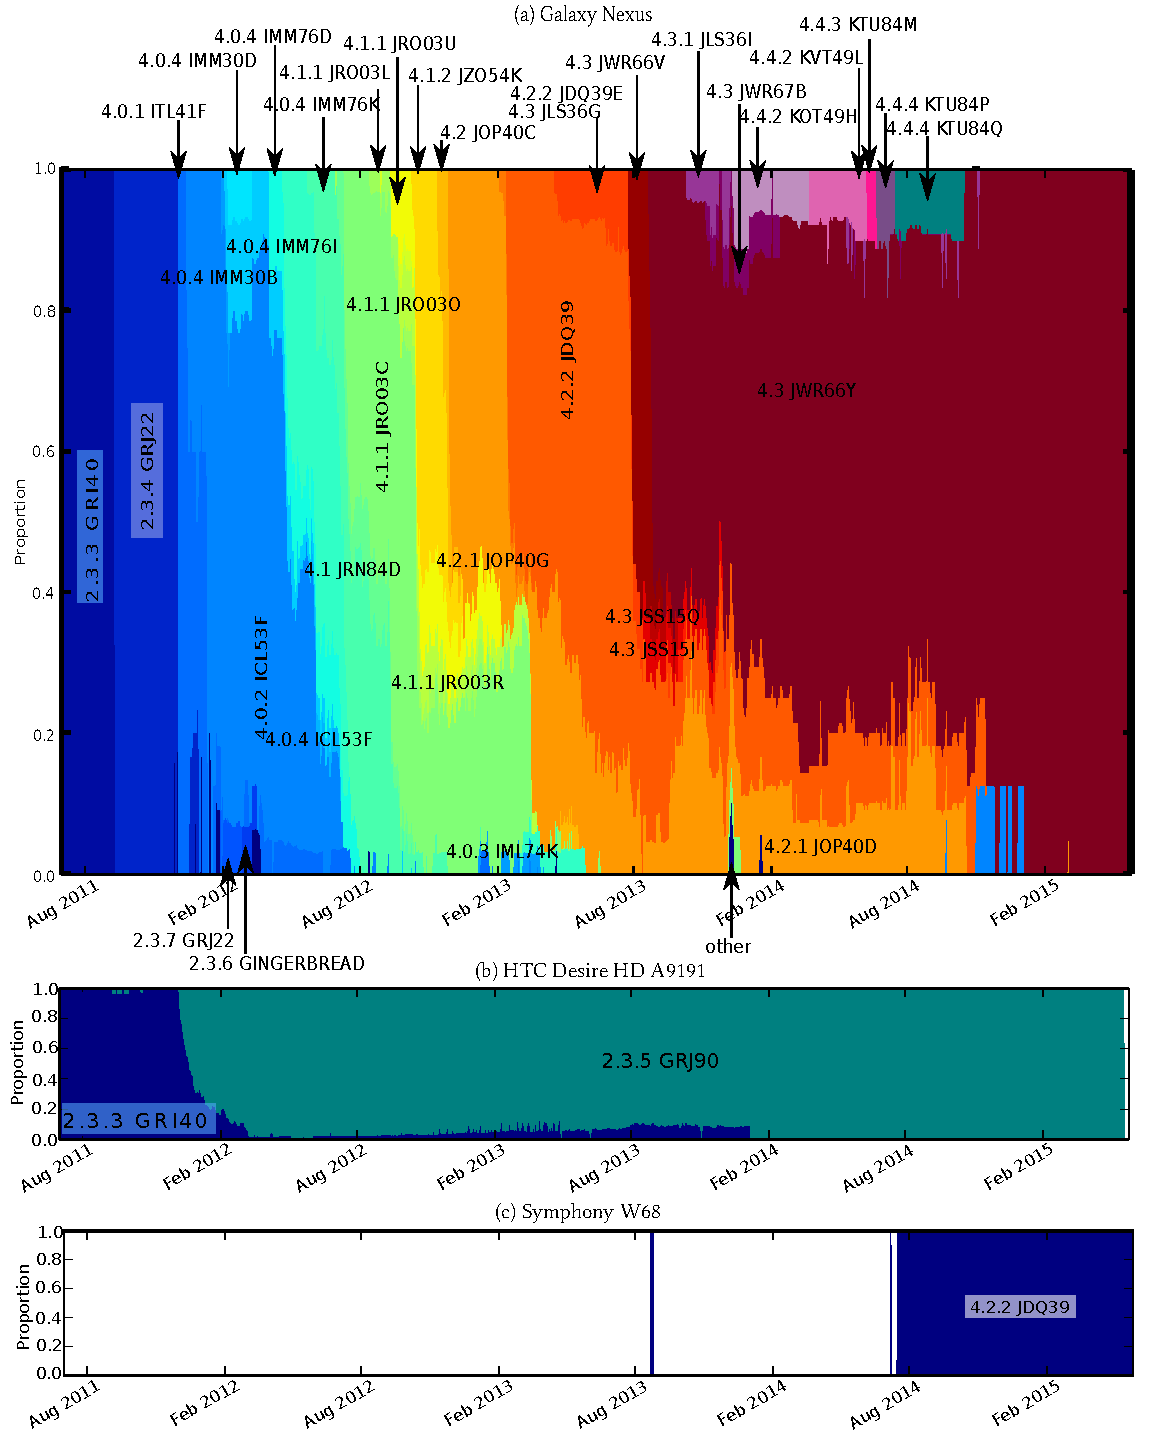
\includegraphics[width=0.9\textwidth]{figures/full_version_comp.pdf}
 \caption{Full version distributions for the highest and lowest scoring models}
 \label{fig:full_version_comp}
\end{figure*}

\daTabSecScoresoperator
We also analysed different network operators, for the \daNumSigOperators\ network operators with a significant presence in our data.
Table~\ref{tab:sec_operator} shows the results \emph{\daSecScoreBestoperator} (\daSecScoreBestoperatorScore\ out of 10) scoring highest and \emph{\daSecScoreWorstoperator} (\daSecScoreWorstoperatorScore\ out of 10) scoring lowest.
However the score of a network operator is affected by the device manufacturers of the devices which are in use on its network.
This is in turn affected by both what devices a network operator offers to users and upon which devices users choose.
Hence having a worse score does not necessarily mean that a network operator is worse, it could be that its users all pick phones from a worse device manufacturer, for example because they were cheaper.
A network operator could use data from this paper to exclude insecure devices from those offered to consumers.
An added value analysis of network operators which takes into account the device mix used by users of that network operator would make it possible to determine whether a network operator is making the situation better or worse by the way it ships updates to users.
However our sample size is too small to do that as while we have significant numbers of devices for each of the device models (Table~\ref{tab:sec_model}) and for each of the network operators (Table~\ref{tab:sec_operator}) we would need a significant number of each model in each network operator.
%We do not attempt to disambiguate users behaviour in whether they install updates from network operators using rolling upgrades.


\subsection{Scores over time}
\begin{figure}
\centering
\begin{subfigure}{\columnwidth}
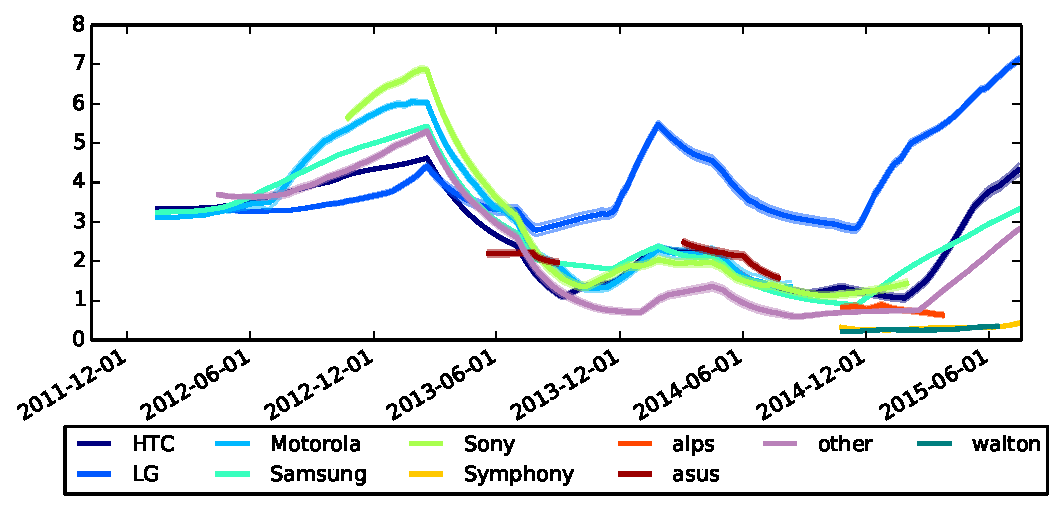
\includegraphics[width=\columnwidth]{figures/security_score_manufacturer}
\caption{Device manufacturers}
\label{fig:security_score_manufacturer}
\end{subfigure}
%
\begin{subfigure}{\columnwidth}
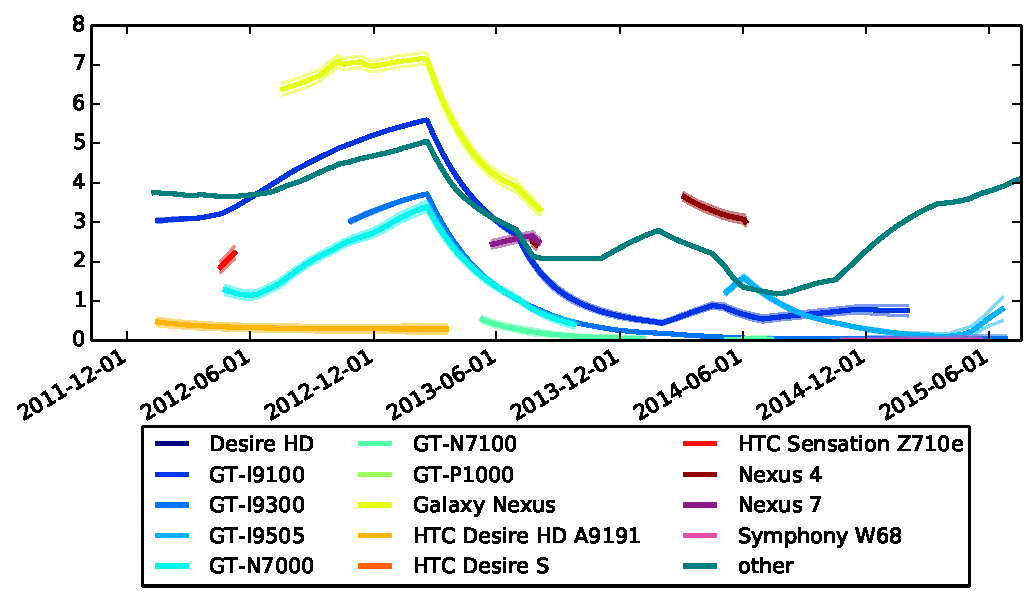
\includegraphics[width=\columnwidth]{figures/security_score_model}
\caption{Device models}
\label{fig:security_score_model}
\end{subfigure}
%
\begin{subfigure}{\columnwidth}
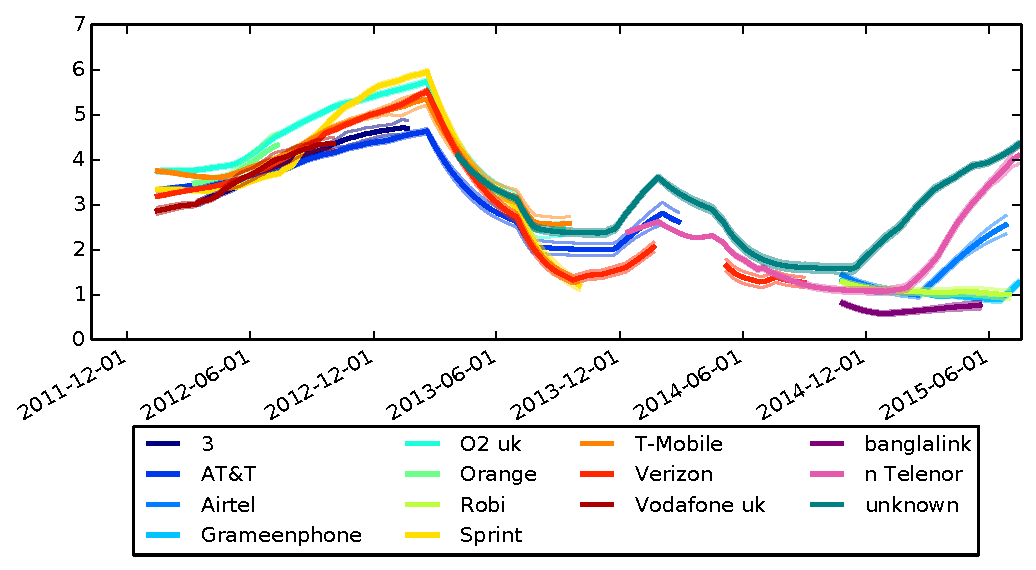
\includegraphics[width=\columnwidth]{figures/security_score_operator}
\caption{Network operators}
\label{fig:security_score_operator}
\end{subfigure}
%
\begin{subfigure}{\columnwidth}
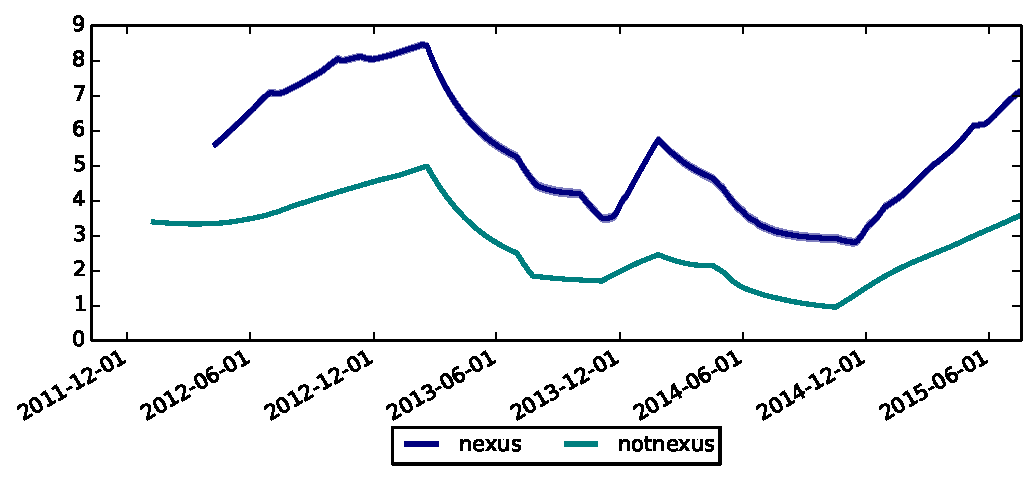
\includegraphics[width=\columnwidth]{figures/security_score_summary}
\caption{Nexus and non-Nexus devices}
\label{fig:security_score_summary}
\end{subfigure}
\caption{Security scores for device manufacturers, device models, network operators and Nexus devices. 95\% confidence intervals indicated.\todolater{bridge gaps?}}
\label{fig:security_scores}
\end{figure}
\todo{This is method rather than result}
The scoring metric as originally computed is averaged over the whole history of the device manufacturer, device model or network operator, it gives equal weight to periods years ago as to in the last few months.
If instead we take an exponential moving average of the daily score for days with more than \daSigNumDevicesDay\ devices when there have been at least consecutive \daSigNumDays\ days of data with that many devices then we can plot how this score has changed over time.
Equation~\ref{eq:rolling_update} shows how the value for a particular day ($v_i$) is computed from the previous day's value and the input for the current day ($n$) with an $\alpha$ of $1/\daSigNumDays$.
\begin{equation}
v_i = v_{i-1} (1 - \alpha) + n \alpha
\label{eq:rolling_update}
\end{equation}
Figure~\ref{fig:security_scores} shows this for manufacturers, device models, network operators and for Nexus and non-Nexus devices.
These show how the scores for different entities are different and change over time, while there is correlated behaviour for different entities (due to things like new vulnerabilities affecting all Android being discovered) these lines still have crossings due to the different behaviour of the different entities.
It also shows that we do not have sufficient data for all the entities all of the time, resulting in gaps in the data.
The clearest results are for Figure~\ref{fig:security_score_summary} with a large gap between the scores for Nexus and non-Nexus devices across the whole data set.


\subsection{Sensitivity of scoring metric}
\daTabDLDistances
\daTabChangeInScores
To evaluate whether the ranking of different manufacturers is sensitive to the form of the scoring metric we computed the normalised Damerau-Levenshtein distance~\cite{Bard2007} between the lists ordered using different forms of the scoring metric, this is shown in Table~\ref{tab:dl_distances}.
The `equal' metric weights $f$, $u$ and $m$ equally rather than favouring $f$ and makes little difference.
Changing the scoring metric also impacts the scores given for each entity Table~\ref{tab:change_in_scores} shows the mean impact on the scores.
This shows that $m$ tends to drag down scores.
\todo{Give some of the actual orderings as well for the most important ones}
\todo{Sensitivity of time based vs. global scores}

\subsection{Gaming the score}
If the comparative data given here is used to influence purchasing decisions then entities in the Android ecosystem might try to game the score rather than genuinely improve security.
$f$ is hard to game without doing a good job at security but it doesn't get any worse if there is already one known vulnerability and another is found.
A high value of $u$ could be achieved by only ever shipping one version but that would give low values for $f$ and $m$ (and not be attractive to new customers).
A high value of $m$ could be achieved by focusing on only one device at a time and ensuring that it gets updates but ignoring all others, but that would lower $f$ and $u$.%
One way to influence our scores would be to add additional devices to Device Analyzer which have good security, these would have to be real end user devices as we could detect fake ones, this would increase the size of our data set and would require providing genuinely good security to some users.
Therefore our score is secure against passive gaming attacks which changed the measured distribution but would require active defence against active gaming attacks which target the measurement devices.


\subsection{Comparison with iOS}
TODO

\subsection{Predicting future version distributions}
TODO

\subsection{Lifetime of a vulnerability}
TODO

\subsection{Monetisation}
%TODO redo this section in light of related work
One of the key differences between smartphones and desktops is that it is easier to directly cash out on a smartphone as malware can send premium rate texts or make premium rate phone calls.
It can also steal personal data which already has semantic information associated with it, this also makes it easier to perform ransomware attacks where malware deletes this information from the device and charges a ransom for its return.
It can also do more conventional things such as use the devices for DDoS attacks and altering the ads displayed to send the fees to the malware author.
While many of these things can be done by malware which just requests the relevant permissions, root exploits make this easier, particularly for ransomware and altering the ads displayed.

\subsection{Incentives and participants}
\label{sec:economics}
\cite{Felt2011}

\subsection{The Device Analyzer data gives a conservative estimate of the Android version distribution}
\label{sec:representative}
\begin{figure}
 \centering
 \begin{subfigure}[b]{\columnwidth}
 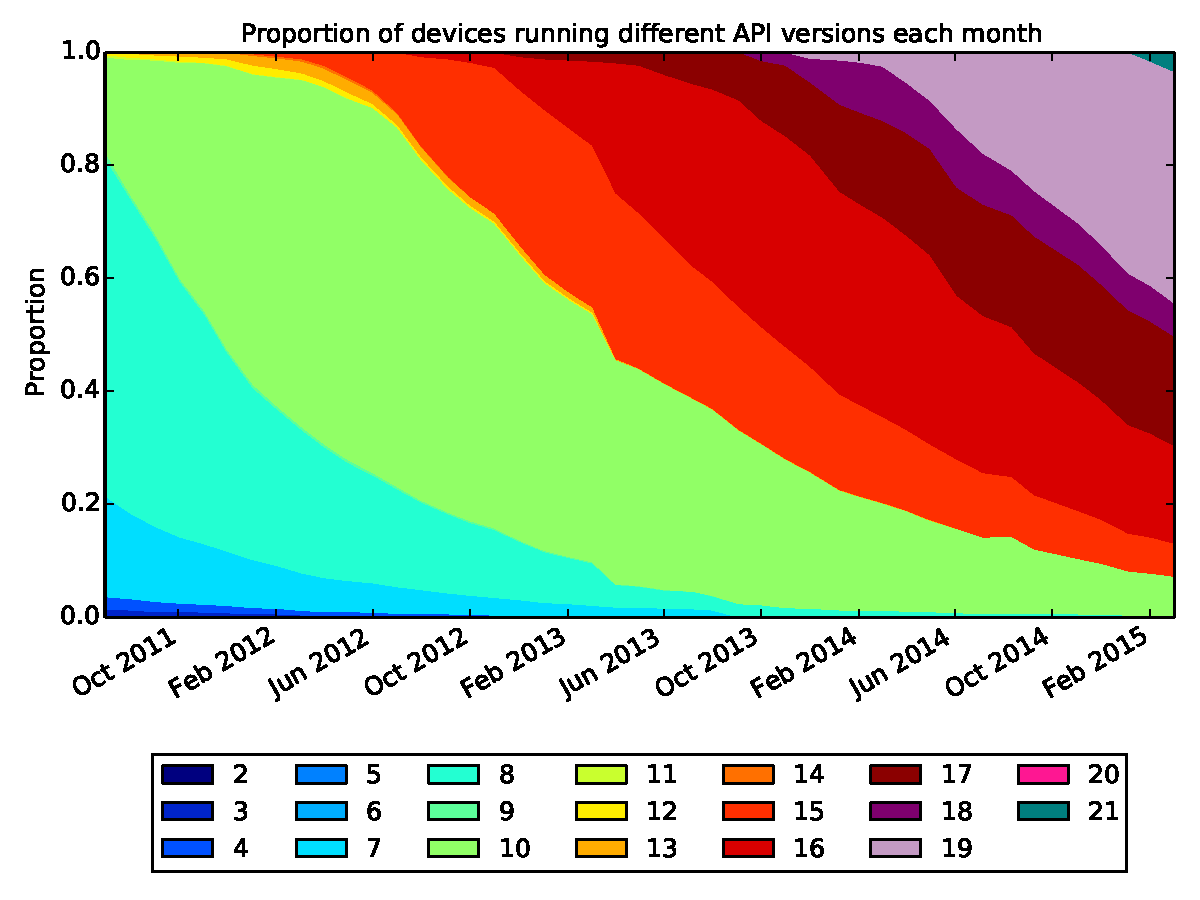
\includegraphics[width=\columnwidth]{figures/googleplayapi}
 \caption{Google Play data on proportion of devices running different Android API versions}
 \label{fig:play_api}
\end{subfigure}
\begin{subfigure}[b]{\columnwidth}
 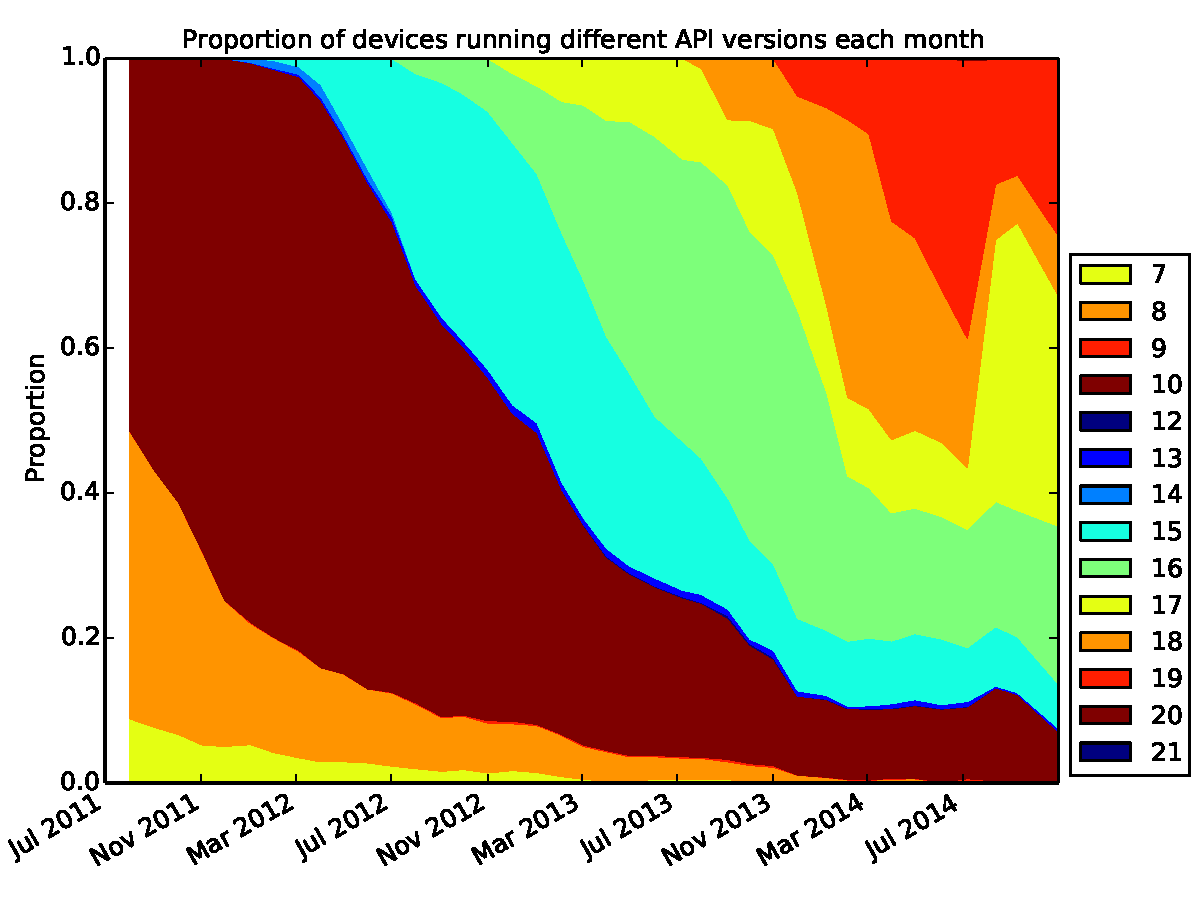
\includegraphics[width=\columnwidth]{figures/norm_api_gpcomp}
 \caption{Device Analyzer data on proportion of devices running different Android API versions}
 \label{fig:da_api}
\end{subfigure}
\caption{Monthly Android API version data}
\end{figure}
\begin{figure}
 \centering
 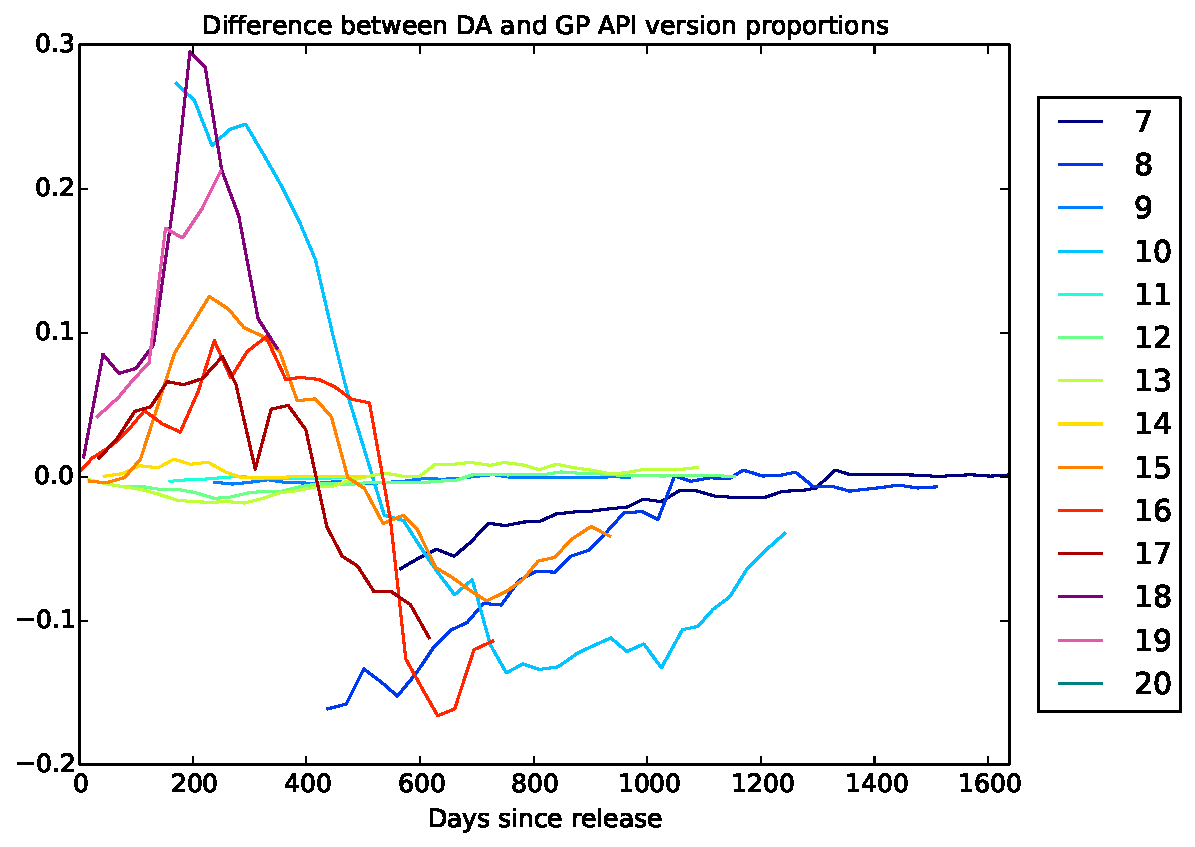
\includegraphics[width=\columnwidth]{figures/api_gpcomp_rdiff}
 \caption{Difference between Device Analyzer and Google Play data on the proportion of devices running different Android API versions}
 \label{fig:da_gp_comp_diff}
\end{figure}
The data from Device Analyzer (DA) we used to investigate the proportion of devices exposed to different vulnerabilities is the OS version.
Unfortunately there is no authoritative source of OS version information and so we cannot check directly whether our data is representative.
However Google has published API version information every month since December 2009 and we have collated this information.\footnote{\url{https://www.cl.cam.ac.uk/~drt24/android/versiondistribution/}}
While API versions are too coarse grained to use for security update detection they are closely related to OS versions and so if the DA data on API versions is similar to the Google Data on API versions then the DA data on OS versions should be representative.
Figure \ref{fig:play_api} shows the data from Google and Figure \ref{fig:da_api} shows the data from Device Analyzer and they appear similar.
Figure \ref{fig:da_gp_comp_diff} shows the difference between Figures \ref{fig:play_api} and \ref{fig:da_api}, normalising for days since the API version was released.
It shows that the Device Analyzer data systematically overestimates the prevalence of new API versions and underestimates the prevalence of old API versions.
This means that the OS version information from Device Analyzer is likely to be overestimating the prevalence of new OS versions and hence our results are a conservative estimate of the security of Android.
%TODO we want a statistical metric to claim this strongly with.
This allows us to have confidence in the OS version information.

\section{Related work}
\label{sec:related}
We found that since 2011 \daMeanInsecurityPerc\ of devices on average were exposed to known root vulnerabilities, in 2011 Felt et al.\ studied 6 Android handsets and found that they were exposed to root vulnerabilities at least 74\% of the time.
This might indicate that over the last 3 years the security of Android has not improved, but these data are not directly comparable.
They also found that 4 of the 46 malware samples (8\%) they analysed contained root exploits, much lower than rates found in later larger studies which found rates of 36.7\%~\cite{Zhou2012b} and 40\%~\cite{Zhou2012a}.
Perhaps the malware authors heard about the results in Felt et al.'s paper?
Our results show root exploits are still a severe threat.

Finding vulnerabilities is frequently a time consuming manual process but, Brumley et al.~\cite{Brumley2008} showed that it is possible to automatically generate exploits from binary patches.
In a similar way some of the vulnerabilities which have been exploited were publicly found by examining the commit made to the Android which fixed the vulnerability.
This effect has been observed before~\cite{Barth2011} in the Firefox source code repositories, Google does not release the source code until after the release of the update reducing this effect to the delay between an update being released and it reaching the last end user device.
There have been other attempts to automatically find vulnerabilities.
The Woodpecker tool~\cite{Grace2012} automatically finds permission leaks in stock Android phone images.
The update process itself can allow Android apps to gain privilege through `Pileup' vulnerabilities~\cite{Xing2014} by registering for new permissions before the update which creates that permission is installed.


There are continuing efforts to reduce the impact of root vulnerabilities, both in Android and more widely.
SEAndroid~\cite{Smalley2013} which is included in Android from version ???~\cite{TODO} claimed to prevent some root vulnerabilities and to reduce the impact of others.
Capability based enforcement systems such as Capsicum~\cite{Watson2010} substantially reduce the capabilities that an exploit has to try and gain increased privilege with.
When Capsicum is included in Linux~\cite{TODO} and hence in Android, it could be used to place fine grained restrictions on system daemons, preventing vulnerabilities becoming root vulnerabilities.

The security protections used in iOS such as only allowing signed code to run, jails and reviewing of apps has resulted in a lower level of malware affecting iOS~\cite{TODO} but can still be bypassed~\cite{Wang2013a}. %TODO look at iOS protections again and tighten this up

Various attempts have been made to detect malware.
RiskRanker~\cite{Grace2012a} classified 3,281/118,318 (2.8\%) apps as risky of which 718 (22\%) were malware and 322 (10\%) were previously unknown, an infection rate of 0.6\% across multiple markets.
It uses signatures of exploits, static analysis of calls to high risk operations, detection of encrypted native code execution and dynamic Dalvik code loading to detect risky apps.
DroidRanger~\cite{Zhou2012a} found 148/182,823 (0.08\%) apps to be malicious across multiple markets of which 29 were previously unknown.
It used permission-based behavioural fingerprinting -- looking at the permissions of known malware and heuristic-based filtering -- dynamic loading of both Dalvik and native code.
AnDarwin~\cite{Crussell2013} detects similar apps, it found 169/265,359 (0.06\%) malicious apps based on the difference in permissions between the malicious app and the app which had been cloned.
It used clustering based on semantic vectors derived from the program dependence graphs to detect similar apps.
The Malware Genome project~\cite{Zhou2012b} collected 1,260 malware samples from 2010--2011.
They found that the best case for anti-malware detection on this data was 79.6\%.
However DroidChameleon~\cite{Rastogi2013} found that antivirus products could not detect malware if it was simply automatically permuted.
All these app analysis projects have been hampered by the difficulty of obtaining full datasets of Android apps as Google does not make these available (and researchers who automatically download them, violate Google's Terms of Service).
PlayDrone~\cite{Viennot2014} was a particularly effective project which circumvented Google's protective measures and downloaded over 1,100,000 apps from Google Play, allowing an in depth analysis.

Examining security updates has been a key way of assessing security for many years.
Many software update systems have been found not to authenticate the connection to the update server and/or do not authenticate the downloaded binaries~\cite{Bellissimo2006}.
Even package management systems designed to provide secure updates have been found to have vulnerabilities~\cite{Cappos2008}.
Fortunately Android does authenticate the update binaries (though the APK vulnerabilities circumvented this) and Google Play downloads them over a secure connection~\cite{Viennot2014}. %TODO double check that

The updatedness rate for Android of \daUpdatednessPerc\ compares unfavourable with the more than 90\% rate for Windows XP SP2 computers contacting the Microsoft update servers~\cite{Gkantsidis2006} though that is within one OS version and only for those computers which did connect to the servers -- but that is the default.

User-Agent strings have been used to investigate how web browser versions change with updates~\cite{Frei2008} and found that at most 80\% of Firefox users were running the most recent version.
The same analysis was used to show that Chrome's use of silent updates seems to increase uptake of upgrades~\cite{Duebendorfer2010} with 97\% of users running the latest version within 3 weeks of release.
Android's update process is manual, the user is notified but must action the upgrade which will then download the update and install it, the phone is rendered inoperable during the update process which is inconvenient for users and the phone must have sufficient charge so that it will not run out during the update process.
Partly this is the result of the fact that an operating system update is being installed and so a reboot is required, but Chrome installs the new version side by side with the old one and switches the next time it is restarted.
The same technique would be more difficult on phones with limited storage space (as for many cheap Android phones which have barely enough space to install just the update) but is a plausible improvement for more high-end devices.
Google is deploying the same silent update technique through Google Play Services~\cite{TODO} which automatically installs updates for core Google components of Android, this also bypasses the manufacturer and operator.



\section{Conclusion}
\label{sec:conclusion}
TODO

\section*{Acknowledgements}
Thanks to David Robertson for helpful advice on statistical analysis.
Thanks to Laurent Simon, Thomas Coudray, Adrian Taylor, Justin Case and Khilan Gudka for reporting vulnerabilities in Android.

\printbibliography

\end{document}
